\documentclass[a4paper,11pt]{extreport}
\usepackage[utf8]{inputenc}

\usepackage{hyperref}
\usepackage{textcomp}

\usepackage{amsmath, amssymb, amsthm}
\usepackage{mathtools, mathrsfs}
\usepackage{bm, bbold, braket, boldline}
\usepackage{cancel}

\usepackage{wrapfig, subfig}
\usepackage{graphicx}
\usepackage{sidecap}
\usepackage{epstopdf}
\usepackage{pst-pdf}
\usepackage{tabularx}
\usepackage{makecell}
\usepackage{setspace}

\usepackage[style=chem-acs, backend=bibtex]{biblatex}
\addbibresource{thesis_ref}

\usepackage[a4paper,
	    margin=2cm,
	    headheight=10pt,
	    inner=3cm]{geometry}
%\onehalfspacing
\doublespacing

\newcommand{\specialcell}[2][c]{%
  \begin{tabular}[#1]{@{}l@{}}#2\end{tabular}}
	
%------------------------------
%		Begin of document		 
		 
\begin{document}


%-------------------------------
%		Title Page
		 
%\frontmatter
\begin{titlepage}

\newgeometry{left=3cm, right=3cm, bottom = 3cm}

\begin{center}
%\begin{figure}[t]
%\centering
%%\includegraphics[scale=0.18]{./images/logo.png}
%\end{figure}
%\bigskip
{\LARGE \textsc{\textbf{King's College London}}} \\
\medskip
{\Large Randall Centre of Cell and Molecular Biophysics} \\
\vspace{0.3cm}
\rule[0.2mm]{\textwidth}{0.2mm}\\
\vspace{4cm}
\huge{\bf Elucidating self-assembly and} \\
\huge{\bf antimicrobial strategies of antimicrobial} \\
\huge{\bf peptides: an in silico investigation.} \\
\end{center}
\vspace{4cm}
\begin{Large}
{\Large{\textbf{Supervisors:}\\
 Prof. Franca Fraternali \\
 Dr. Chris D. Lorenz}} \\
\vspace{0.5cm}
\begin{flushright}
{\Large{\textbf{Student:} Irene Marzuoli}}
\end{flushright}
%\vspace{20mm}
\end{Large}
\begin{center}
\vspace\fill
\rule[0.2mm]{\textwidth}{0.2mm} \\
{\large{\textbf{2019}}}
\end{center}
\end{titlepage}

\restoregeometry

%\tableofcontents


%-----------------------------
%		Abstract
%\Large{
%	\abstract{
%		\large{
%
%		}
%	}
%}



%-----------------------------
%		Main body

\chapter{Introduction}

%\begin{wrapfigure}{R}{8cm}
%\centering
%%\includegraphics[width=70mm]{figures/res_insurgence.jpg}
%\caption{Deaths per year due to different causes and projection up to 2050 for AMR casualties. Data from 2016 Review on Antimicrobial Resistance \cite{am_rev}.}
%\label{fig:AM_resistance}
%\end{wrapfigure}

%PICTURES
%1 many drug delivery vehicles (collage mio)
%2 plot/table on resistant antibiotics
%3 Some structure of AmPs (beta, alpha, ...)
%4 mech of action AMPs
%5 picture of LFC e some results from experiments
%6 triskelion and capzip
%7 exp results preliminary


\paragraph{[Why: philosophy]} Add some refs but not read yet.
% REF:
% AlphaGo, AIreview, Rossi2018, history_medicine_review, other_review_early_drugs?, drug_database, review_drug_delivery, WIDES_database, ABX_database_jhopkins, Mitchess1945, Strebhardt2008.

Theory stays to experiment as experiment stays to nature. And science stays to technology as technology stays to life.

To navigate this huge gap is the scientist call, in an effort to bring the extremes closer, giving a model of how nature functions, or to enrich the space in between, inventing new realities. Technology bridges every day this very gap: every consequence of our abstract thinking is technology, an hidden layer of inductions and deductions which brings us from abstract principle to solutions. Computers, the ultimate technology, are emulating increasingly better and more efficiently this process, sparing us the awareness of the complex mechanisms which thread the problem to its solution. It was in the past two centuries that we witnessed such an evolution of techniques, inventions and machineries that we can now exploit years of theoretical thinking by using tools in practical problems to eventually modify nature in every daily activities. If in the past nature was the mystery and the human intervention on it was simple to understand, now on the contrary many basic principles of the physics laws are clear to most of us but human inventions became increasingly complex, condensing centuries of discoveries in simple, efficient tools. We use planes, drugs and the internet not because we perfectly understand how they work, but because we trust the collective knowledge we, as humans, have accumulated so far.

Out of the many fields at service of the humanity wellness, the most challenging and still far away from being exhausted is the understanding and manipulation of the human body and mind. While machines - in the broadest sense possible - can perform actions in our place, they can't yet think and live on their own. It is striking how we are finally scratching the understanding of these two entities, mind and body, in the same historical moment, at a point where computers imitates the human reasoning \cite{AlphaGo, AIreview} and biological materials are turned into semi functional organs \cite{Rossi2018}. However, we are far from completing the jigsaw of knowledge on these topic. On the contrary with the progression of the techniques available to investigate various fields, we realise how vast is the space to be explored. It is then a logical consequence that the modern scientist is becoming more and more specialised, drifting away from the comprehensive knowledge owned by scientists up to two centuries ago; but exactly because the full picture is challenging, every project aimed at understanding an aspect of these enormously vast themes, no matter how tiny the subject is, is involved in a network of efforts, in the hope and trust that piecewise knowledge can build a unique and organic corpus.

This thesis places itself in the domain of understanding how the human body works - how the (non) equilibrium of life is possible and how human intervention can be possible. The tiny and narrow topic it covers wants to explore one possible way in which we help the body to heal itself and to defend itself against external malicious agents. To correct those processes that go wrong means life, and we are biologically and emotionally pushed towards actions that prolong and improve life and have always looked at ways of curing ourselves. But the body evolved in the past blind to reason, on the contrary taking advantage of multiple defences and barrier which secured it from the failure of the reasoning, and it is know to us often a mystery, as we struggle to understand many of its components, letting aside the whole picture.

Quite blindly then we developed in the past a medicinal science which managed to be of service to the human envelope, in what was a remarkable game of trial and error resorting to magic first and to our intelligence last \cite{history_medicine_review}. The risk and inevitable failures tracing the path were a necessary toll to the utmost necessity of keeping healthy, safe and - ultimately - alive. In a history resembling the evolution of technology, we resorted to nature for beneficial molecules \cite{above}, which we called drugs in the initial fuzziness existing between healing and deadly, but then humans started identifying the beneficial principle in these natural remedies \cite{other_review_early_drugs?}, and ultimately to produce new molecules \cite{other_review_early_drugs?}. The increasing understanding of how we worked pointed out the many challenges a drug has to withstand to be efficient. And this knowledge poses question: if so many barriers prevent a drug from entering the body, how can infectious agents have found a way to our cells? And if we want to fight those ones instead, why the body cannot recognise these helpful molecules as beneficial ones and is fighting them instead? Are they perhaps damaging for us as well, in some way we have not yet understood?

Luckily, if knowledge has brought awareness of the complexity of the machine our body is, it started bringing also solutions. We do now have drugs \cite{drug_database}, we know how to selectively deliver some of them \cite{review_drug_delivery}. We have disinfectants \cite{WIDES_database}, and we have antibiotics to fight pathogens \cite{ABXdatabaseJhopkins}. We do know what we are composed of \cite{Mitchess1945} and how this material rearranges in organelle, cells, organs. And we know some of the mechanisms concerting these parts together \cite{what?}.

We are finally moving in the direction of the magic bullet envisioned a century ago by Nobel Prize Paul Ehrlich, who dreamed of a 'personalised and tailored drug' able to target specific molecular defects while being harmless - if not beneficial - to the other cells.\cite{Strebhardt2008} Such success would condense in a tiny amount of space a century of efforts in understanding the human body. But we still miss many pieces of information as the more we zoom in, the less each single researcher can monitor at once and the more we realize is there to be discovered.

In this prospect, looking at how one particular molecule behaves with respect to a particular environment, as this thesis does, using a simplified theory (sometimes the only possible) is certainly a tiny fragment of knowledge added to the world of science. But, joint to the other scientific output from the community, it is a necessary, meaningful and promising fragment.

\vspace{2cm}
This introduction is meant to give an overview of the many different challenges the fields of medicine and bioengineering have faced in recent years, challenges that have arisen the interest for self-assembling antimicrobial peptides. Antimicrobial peptides were not a primary source of interest in these fields as other materials and concepts were deemed more suitable to solve the tasks coming along the way. It is therefore important to clarify the landscape of such other solutions and approaches to understand and value why a change in the research focus has come to age. Figure \ref{fig:intro} provides a workflow of this introductory chapter to help the reader in identifying the sections of interest.

\begin{figure}
\centering
\Large{\textbf{Motivations of the work: a graphical abstract}}\par\bigskip
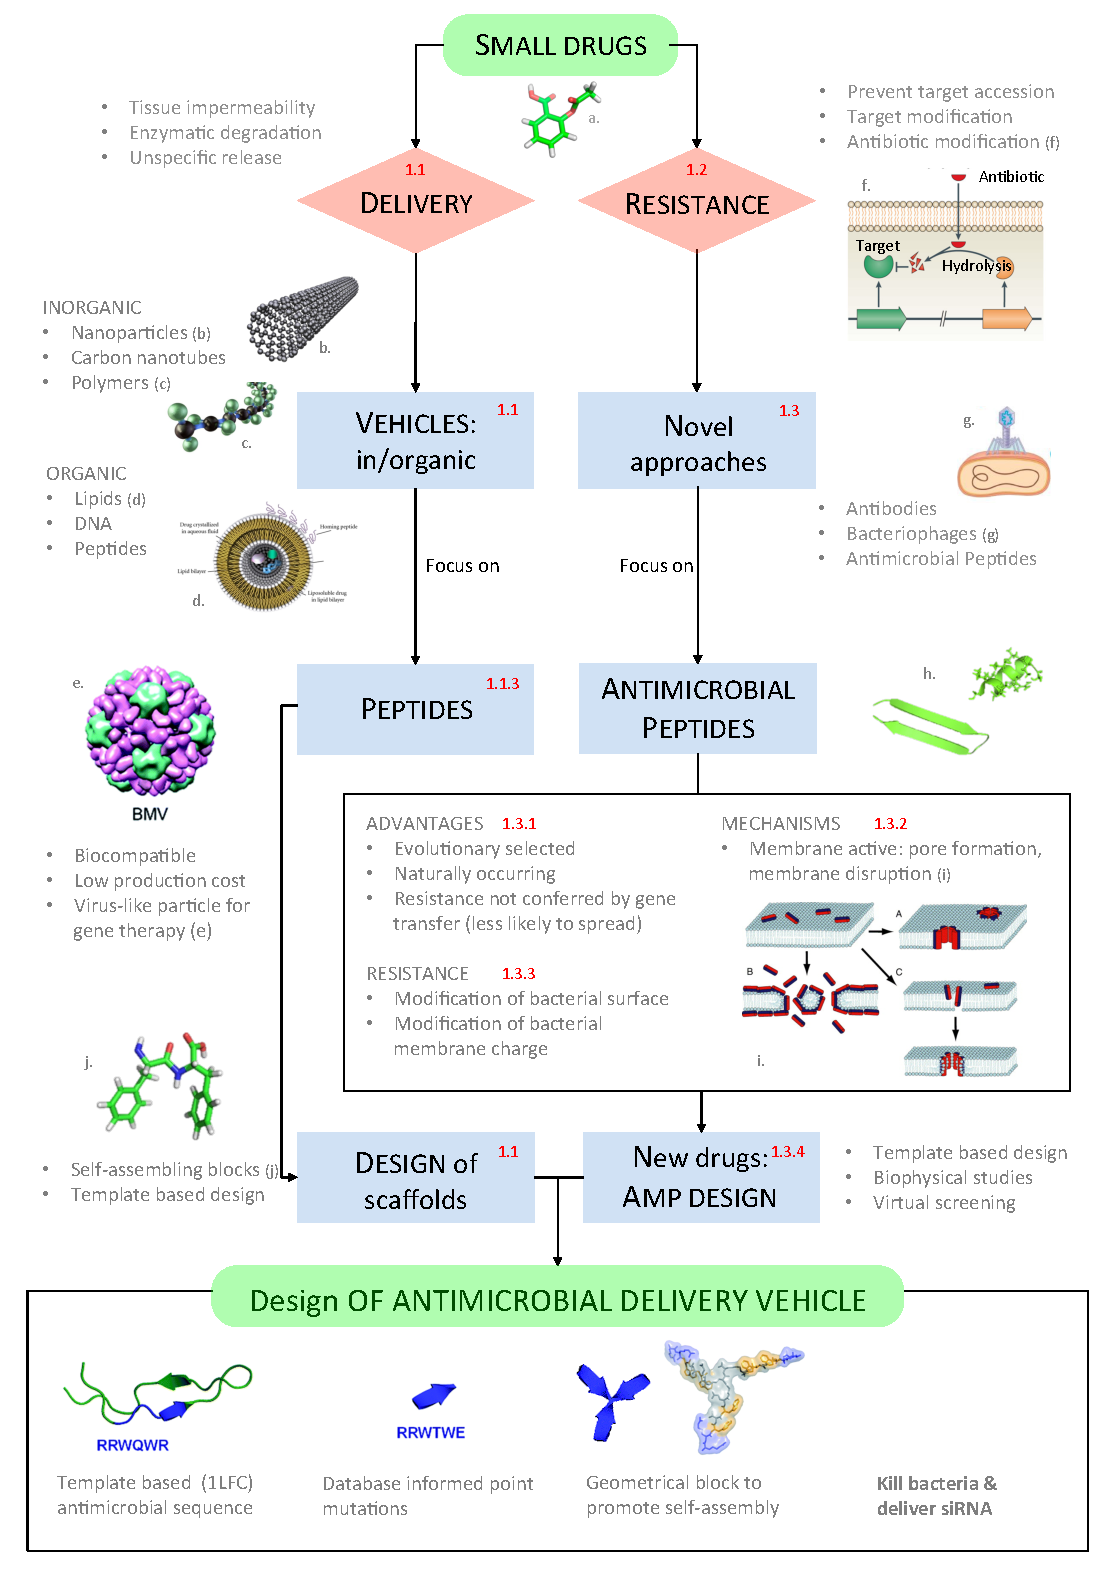
\includegraphics[width = \textwidth]{pics/scheme_intro}
\caption{Figures a. to k. adapted from: a. [11], a. [11], a. [11], a. [11], a. [11], a. [11], a. [11], a. [11], a. [11], a. [11], a. [11]} \label{fig:intro}
\end{figure}

\clearpage


\section{Drug delivery: challenges and solutions}
% REF
% Masaoka2006, Mitragotri2014, Krol2012, Pattni2015, Jain2016, Mitragotri2014, Hughes2005, Singh2018, Astruc200, Erol2017, Depan2011, Lammers2009, Liechty2010, Kawakatsu2001, Julien2013, Lakshmi2007, HarshaRao2018, Yoo2011, Yingchoncharoen2016, Bunker2016, Pattni2015paper, Jain2017, Linko2015, Douglas2012, Zhang2014, Jiang2012, Refvirusbehaviour, Lauer2017, Daya2008, Buning2015, Smalley2017, Wu2010, Fan2017, Habibi2016, Ma2012, Yan2010, Silva2013, King2014

\subsection{Environmental challenges of drug delivery}
The problem of drug delivery is an excellent example of the hurdles existing between a theoretical reasoning and nature: a new drug is usually designed to affect a specific target. Even if in silico experiment can prove its efficacy, its usefulness is bound to its ability to cross the many barriers dividing the inoculation site from the very target inside the human body.
%
To reach the aimed organ, drug molecules must be compatible with the different cellular environments they cross but be preferentially retained and act only on the ones they are designed for. This implies a subtle balance between a disruptive activity on one side, and harmlessness on the other, least the compound is recognised as dangerous and disposed of by the efficient immune and reticuloendothelial systems of the body which aim at neutralise every exogenous substance.

As en example, the trip of an orally  administered ``free" drug, i.e. an active molecule without any aiding delivery agent, passes through the digestive system, with its challenging acidic environment and limited permeation across the intestinal epithelium, and from there to the blood stream.\cite{Masaoka2006, Mitragotri2014} Then the drug diffuses in the tissues flanking the blood vessels naturally depleting its concentration downstream,\cite{Krol2012}  so that regions further away in the line have less chances of getting a sizeable dose, which implies that high drug concentrations might be needed as starting point to efficiently target every organ.

However, this naive picture of a drug diffusing in the body is complicated by the impermeability of specific tissues: the brain for example, one of the most delicate organs in the body, is well protected from the attack of external agents by the blood brain barrier (BBB), which allows the passage of small molecules only ($<$ 400-500 Da, while standard 'small molecule drugs' go up to 900 Da) of high lipid solubility \cite{Pattni2015, Krol2012}. Other tissues, like tumoral ones, are instead poorly vasculated, reducing the chances of delivery at their interior.\cite{Pattni2015}

Finally, during their journey to reach the receptor, enzyme or organelle they are meant for, drugs must not be captured and disposed by the immune systems. However, inorganic small molecules are not mimetic by themselves, i.e. they often do not resemble the ones naturally present in the body, and this brings uncertainty on how they would interact with organic molecules. Generally, as soon as they reach the blood stream they are coated by a protein corona based on their shape and charge.\cite{Krol2012} Such modifications are often difficult to predict and can disrupt of decrease significantly the efficacy of the compound as they modify the way drugs are recognised and absorbed by the target. 

For all the above reasons, research has focussed on developing systems to assist the delivery of drugs.\cite{Jain2016, Pattni2015, Mitragotri2014} A mimetic carrier can not only improve delivery, but also be designed to selectively bind to particular tissues or to trigger the drug release after a given time or upon changes in environmental variables (for example pH) to reduce drug concentration in non targeted regions. A stand alone field of research has then focussed on the development of delivery vehicles irrespective from the quest for disease targeting compounds. The optimised products of the two efforts can then be paired according to the condition to address.

At present, many molecules have been successfully employed to build drug vehicles: inorganic metals, polymers, lipids and proteins are all suitable for the aim and offer a range of different physico-chemical characteristics useful to target different regions.\cite{Hughes2005} A brief overview of them is meaningful to point out the broad variety and exoticity of structures which can be useful in the medical world, sometimes unexpectedly.


\subsection{Inorganic materials for small drugs delivery}

\paragraph{Metal nanoparticles} In the range of inorganic compounds, golden nanoparticle demonstrated to be remarkable for tumor treatment: first of all, they can be customised in shape and size (down to a 10 nm radius), coated with biologically active moieties or made less visible to the immune system by conjugation to a poly-ethyleneglycol (PEG) polymer layer.\cite{Singh2018} Moreover they possess optical properties that allow them to be tracked inside the body and they can be thermally stimulated to trigger the release of drug, favour the penetration through the cell membrane or perform thermal therapy, disrupting the cells nearby.\cite{Boisselier2009} At present, there are mixed evidence about their toxicity\cite{Boisselier2009} and doubts have been raised on the long term effects of metallic fragments in the body. For that reason, only a few golden nanoparticle based compounds have made to the clinical stage so far\cite{Singh2018} but, given their high and still unexplored potential, they continue to be a primary interest of the medical community and a very active research field.

\paragraph{Carbon nanotubes}
Similarly, carbon nanotubes have been used for biomedical applications as they have a high loading efficiency thanks to their high surface area and easy interaction with biomolecules through van der Waals, $\pi$-$\pi$ stacking or hydrophobic effect.\cite{Erol2017} Therefore they are easy to functionalise through conjugation to extra organic groups to increase their biocompatibility; and have potential for targeted drug release upon change in environmental pH.\cite{Depan2011}

\paragraph{Polymers} Polymers are another large class of inorganic molecules functionalised for the benefit of medicine: for example PEG has already been mentioned as aid to make golden nanoparticles bio-compatible. Indeed, thanks to its high hydrophilicity, it is a clinically approved molecule widely used to mimetise structures (e.g. inorganic, peptides) which in turn carry a drug,\cite{Lammers2009} or as a stand alone carrier system, as it has a high drug payload.\cite{Liechty2010} As each of their monomer constituent can be either hydrophilic or hydrophobic, the great strength of polymers is their flexibility. They can be engineered to assemble in many different structures,\cite{Kawakatsu2004}; they can trigger a sustained drug release by swelling slowly in water,\cite{Nicolas2013} or undergo sol-gel phase transition upon specific changes in the environment.\cite{Liechty2010} Finally, research has also focussed on improving their biodegradability\cite{Nair2007} or in making polymers a bioactive compound itself.\cite{Rao2018} [toxicity? Better for oral absorption?]


\subsection{Organic materials for small drugs delivery}

A somehow opposite approach for designing drug vehicles to the use of inorganic material consists in using molecules similar to the ones present in the body, in an effort to exploit already available biocompatible materials and reduce toxicity.\cite{Yoo2011} In this category fall lipids, DNA and peptides.

\paragraph{Lipids} Lipids are the main constituents of the cell membrane and as such they represent a mimetic material. They come with a great variety, enhanced by the many species produced synthetically. The components selected for drug delivery are usually taken from the biological lipidome, but their composition differs from the cellular membrane one, and possibly includes synthetic molecules, to tune their release properties and enable them to survive the delivery journey.\cite{Yingchoncharoen2016} They can encapsulate efficiently both hydrophobic or hydrophilic drugs, arranging themselves in micelles structures (monolayer spheres with the hydrophobic tails facing the interior) or in liposomes (bilayer spheres with a water filled core),\cite{Bunker2016} with many of them overcoming the clinical stage and currently approved for cancer and infections.\cite{Pattni2015paper, Jain2017}

\paragraph{DNA scaffolds} Similarly, many DNA scaffolds have been tested for smart delivery: DNA origami is nowadays an established technique to build three dimensional customised solids\cite{Linko2015}, and the nanometric knowledge about their constituents makes possible fine tuning them for a triggered release of the content.\cite{Douglas2012} First studies proved them successful in delivering anticancer agents,\cite{Zhang2014, Jiang2012} however they are very sensitive to cellular environment and this, united with high production costs, prevented them constitute a viable class of carriers so far.

\paragraph{Peptidic scaffolds} Another widely used and trustworthy mimetic vehicle comes, quite surprisingly, from the world of pathogens: viruses have co-evolved with humans, to be able to penetrate into cells where they complete their reproductive cycle\cite{??} Therefore their capsid, the peptidic shell encapsulating the genome, is highly suitable for cell penetration. The first application sought historically was to employ genome free viruses to stimulate and train the natural immune response against the respective genome-loaded ones, creating viral vaccines - in a similar fashion to what already done with the inoculation of dead bacteria to counteract the infections caused from them.\cite{Lauer2017}
Later in the history, their potential as cargo carrier was pursued first by modifying their genetic material to include sequences beneficial for the host cell and prevent the infectious duplication at the same time. In particular the adeno-associated virus (AAV) has been widely studied\cite{Daya2008} as it triggers a low immune response,\cite{Buning2015} and the first AAV viral therapy has been finally approved a few years ago.\cite{Smalley2017}
%
To fully exploit the potential of a peptidic carrier many efforts have focussed on synthesising in vitro gene-free capsids, either as they appear in nature\cite{Wu2009} or designing artificial building blocks, which assemble in  so called Virus-Like particles (VLPs), to help overcoming the reaction stimulated by specific viral capsids to which the immune system is (already) sensible to.

Among their advantages, peptides present biocompatibility, a low production cost and a tunable bioactivity thanks to their chemical diversity, which help in tailor the assembly toward the target of interest.\cite{Fan2017} Moreover, the variety of amino acid available makes possible to load peptidic structures with both hydrophilic and hydrophobic drugs, according to their amino acid composition.\cite{Habibi2016,Ma2012}
%
Similarly to other delivery vehicles, the surface of such particles can be functionalised with additional molecules to improve the target selectivity and increase biocompatibility, while the peptidic scaffold grants robustness to the structure. Therefore, VLPs loaded with drugs can be tuned for an efficient intra cellular release.\cite{Ma2012}
%
The easy manipulation of peptidic structure derives from the fact that proteins are a fundamental component of the human body, so that there is a vast literature on their interactions with membranes, cell receptors and in general biological components, from which the design for novel materials can take inspiration to employ building block sensible to particular triggers within the body.

A step further in engineering peptidic structures is represented by the design of self-assembling functional structures from first principles, i.e. to exploit the physico chemical characteristics of peptides, regardless their resemblance of viral capsids.
%
Indeed self-assembling peptides can form nanostructures ranging from nanoparticles to nanotubes, nanofibers, nanorods and hydrogels.\cite{Fan2017,Habibi2016} The assembly is modulated by the peptide length and its hydrophobic or hydrophilic character: on one end of the length scale, phenylalanine dipeptides were designed with inspiration of a pathogenic process towards molecular self-assembly\cite{Yan2010} and were shown to self-assemble in a multiscale process producing nanotubes able to load drug molecules.\cite{Silva2013} The relatively small diphenylalanine building block is non the less complex has it bears two charged termini (as the process is observed at neutral pH), and two aromatic hydrophobic rings, therefore the dipeptide is driven towards assembly by the hydrophobic forces acting on the phenylalanine side chains.

In a different approach, longer sequences can be employed to guide the formation of the local structure, as they organise spatially in well studied motives (the secondary structure) with a known interaction among themselves.
%
The two typical secondary structures, $\alpha$-helices and $\beta$-sheets, appear in sequences of about 20 or more amino acids length and are both amphiphatic, thus promoting the assembly between the hydrophobic faces of different copies of the same structure. With the appearance of a secondary structure, more complex building blocks can be designed, to tune the shape into the ones needed for the supramolecular organisation of interest.\cite{King2014} Again, the knowledge of many protein structures\cite{PDB} give us insight in how the small structure can hierarchically assemble into larger ones - however the challenge and outlook often goes in the direction of synthesising exotic, non natural, novel geometries.\cite{Yeates2019,Malay2019}


\section{Challenging the small drugs scenario: antimicrobial resistance}

% REF
% Santos2017, McKellar1999

The previous brief review on drug carriers rotates around the paradigm that a drug is a small molecule inorganic compound (of mass up to 900 Da) which targets a specific molecule of a specific target of a mammal or bacterial cell. In this light, the ultimate goal of the delivery vehicle is to carry the drug to the site of action where it can interfere with the processes it is assigned to. Very often the target of interest of small molecule drugs are proteins: out of the 695 small drugs approved by FDA (the American Food and Drug Administration agency) to target human molecules, 667 acts on proteins. Similarly, 189 of the 198 small drugs approved to treat pathogens have a protein as their target.\cite{Santos2017}
%
It must be noticed however that the identification of an unambiguous drug target poses challenges in many cases, especially when the drug binds to a protein complex or to a number of closely related gene products.\cite{Santos2017}

In presenting the aforementioned figures, the data were naturally split among the drugs which target human molecules, ``repairing" some faulty process in the human body, or the ones active against bacteria, which ``disrupts" the bacterium life cycle in order to kill or prevent the reproduction of the pathogen.
%
It appears evident that the pool of drugs available to the second purpose are in consistently lower number than the ones addressing human molecules. This comes from the nature of the action they perform: molecules targeting human proteins need to be highly specific to avoid interference with other proteins or with healthy cells, and in a sufficient number to address the variety of diseases affecting the human body.
%
Antibiotic must be non-toxic for human cells as well, i.e. their target must not be shared between mammal and bacterial cells,cite{???} but there is a less stringent requirement in their selectivity on different bacterial species. On the contrary, it is often useful to have a broad-spectrum compound. This cross-species efficacy and non-toxic property is obtained thanks to the evolutionary relationship among bacterial species, and between bacteria and humans: while the first are closely related, and therefore share homologous proteins with very similar structures, humans have less architectures in common with them, allowing for a resilience against bacteria-targeting drugs.\cite{???}
%
Of course the set of bacterial species is very diverse and the cross-species effectiveness of some drugs does not extend to the whole bacterial population. This demonstrates to be a positive feature, given the large amount of beneficial bacteria that live in symbiosis with the human body (especially in the gut\cite{???}) and that must be preserved for an optimal wellness.

In the framework described above, it is understandable that the first time research on antibiotics was satisfied with the development of a handful of potent, broad-spectrum compounds.
%
Penicillin, the first of them, was isolated from a mould in 1928 by Alexander Fleming. It acts inhibiting the formation of peptidoglycan cross-links in the bacterial cell wall (for a review of bacterial cell membrane structure the reader can refer to Section -- and the relative references). This inhibition is achieved through binding to the enzyme DD-transpeptidase responsible for the catalysis of such cross-link.\cite{McKellar1999???}
%
As foreseen from Fleming himself in his Nobel Prize acceptance speech, bacteria can become immune to penicillin, and this is specifically achieved by either production of penicillase, an enzyme that degrades penicillin, or by subtle changes in the structure of the penicillin-binding proteins to prevent penicillin binding or again by removal of the drug outside of the cell through specially re-purposed efflux pumps that they use to release substances from the cell.

\subsection{Course of antimicrobial resistance} \label{sec:course_AMR}
This mechanism is not an exceptional characteristic of penicillin, but only one example as many drugs became less effective since their discovery till nowadays. In the first stages of the insurgence of antimicrobial resistance (AMR), less effectiveness of a drug means that some strains of bacteria are not damaged by the standard doses of the drug as they possess some natural occurring mutations in their genome which promote an escape mechanism which invalidate the drug effectiveness.\cite{Kapoor2017,Blair2014} Usually only a small population of bacteria is resistant, and it can be killed never the less by augmenting the dose of the drug. However, the natural course of AMR states that the resistant population will replicate faster that the peers of the same species because it is more fit in an environment challenged by the presence of the drug. It is noteworthy that this fitness might not be optimal in a natural drug-free environment - and indeed the wild population has not been selected for that genotype - but under the pressure derived from the treatment, other characteristics result more advantageous.
%
In the short time scale it is usually sufficient to increase the doses of a drug to re-gain efficiency against the target, but it has been observed that a species resistant to a drug can usually adapt to higher doses of the same.\cite{????} Moreover, high drug doses are not always applicable due to the severe side effects they are connected to.\cite{????}

The spread of resistance between bacterial cells and even species is very effective as bacteria are able to exchange genetic material with other individuals via small rings of DNA in a process called conjugation.\cite{????} In this way the advantageous characters which promote resistance spread across individuals and species with an innate resistance can transfer to other ones their mechanisms of resilience to a particular drug.
%
Therefore, despite AMR is an evolutionary mechanism, the fast pace at which bacteria replicates, their enormous population (in terms of individuals), and the relative easy horizontal gene transfer through conjugation place the insurgence of resistance well within the human lifespan time scale.\cite{????}

It is then clear that resistance is a very complex problem which depends on many variables: the casual appearance of resistant individuals, the transfer of information between them, the relatively larger fitness of resistant individuals and the dosage and time line of the drug administration. Many mathematical models have been implemented to understand the issue\cite{Birkegard2018,Niewiadomska2019}, but it is known that some particular strategies of drug administration are worse than other, favouring the proliferation of resistant bugs.
%
One example is the underdosage of antibiotics: a low drug load is likely to harm but not kill pathogens, in particular to promote the fitness of resistant ones. In a sort of ``gym" or ``vaccination" process for bacteria, an underdosed drug would kill the weakest individuals but strengthen the resistant population, which would now be fitted to the challenges of a higher dosage.\cite{????}
%
Similarly, the abuse of antibiotics puts an high pressure on the pathogenic populations, which is desirable but at the same time can induce a faster emergence of escape mechanisms.\cite{????}
%
In this context it must be noticed that many drugs are bacteriostatic agent as opposed to bactericidal: i.e. they prevent the bacterium growth rather than kill it, as they are meant to control the bacteria and slow down the damage while host defence mechanisms to eradicate them.
%
It is then clear that a high dosage of a bactericidal agent may to extinguish the bacterial population and eradicate the disease, but for bacteriostatic drugs, once they are removed, bacteria can usually start again their reproduction cycle.

It is noteworthy that abuse of antibiotics can take many forms: a part from the drugs used to treat human related diseases, the agricultural and breeding sectors are constantly using antibiotics to keep their products secure form illness. This results in large quantities of drugs to be released in the soil and water, which ultimately reach humans in underdosed quantities. Diseases of plants and animals are different from the ones affecting humans, however some drugs are effective on many bacteria including the one affecting humans. Therefore the widespread use of antibiotic for animals or plants can ultimately lead to train resistant bacteria in humans.\cite{????}
%
Additionally, the diseases can cross species: this means that an extra care must be taken in the treatment of non human bacteria least to promote resistant ones which can at a point cross species and affect us.\cite{????}

The complexity and severity of the issue is such that it has been raised to the status of national emergency in several countries, including UK, as we are leaving the century in which antibiotics were discovered, to enter a phase in which we count the number of the ones loosing efficacy.\cite{Oneill2016}

REDO: SAY THAT IT MAKES SENSE THAT SOME BEHAVIOURS TRAINS BETTER RESISTANT BACTERIA, AND THAT THIS IS A SOCIAL EMERGENCY??


\subsection{Mechanisms of antimicrobial resistance to small drugs} \label{sec:AMR_mechs}

Antimicrobial resistance can manifest through many different mechanisms, as highlighted in the example of the penicillin resistant bacteria.
%
In particular, resistance mechanisms fall into three main groups: a first group minimises intracellular concentration of the antibiotic preventing penetration of maximising efflux; a second one modifies the antibiotic target by genetic mutation or post-translational modification; finally a third group inactivates the antibiotic by hydrolysis or modification of the drug molecule.\cite{Blair2014}

\paragraph{Prevention of access to target}
One possible mechanism of defence bacteria employ against antibiotics is to prevent the access to the target. This is performed either preventing the drug influx or promoting its quick efflux in the eventuality it has entered the cell.

Regarding drug influx, not all the molecules can enter the cell permeating the membrane, and this holds particularly for hydrophilic antibiotics tackling Gram-negative bacteria: indeed, compared with Gram-positive ones, Gram-negative bacteria are intrinsically less permeable because of the structure of the additional outer membrane,\cite{Delcour2009} therefore hydrophilic molecules are imported into the cell through outer-membrane porin proteins.\cite{Vargiu2012,Kojima2013}
%
The major porins of most Enterobacteriaceae are thought to be non-specific channels,\cite{Tran2013} therefore, replacing porins with more selective channels or down regulating their expression would limit the intake of the drug. This last mechanism is well established and contribute to resistance to many different drugs in Gram-negative bacteria, including newer drugs such as carbapenems and cephalosporins, for which resistance is usually mediated by enzymatic degradation,\cite{Tamber2003,Baroud2013,Lavigne2013,Poulou2013,Wozniak2012}
Finally, in E. coli exposed to carbapenems, not only the porin expression is down-regulated, but also the genes coding for porins are heavily mutated, suggesting that changes in the porin structure can enhance their selectivity and reduce the drug influx.\cite{Lavigne2013,Novais2012,Tangden2013}

A strategy complementary to prevent drug influx is to dispose of the drug efficiently once it has invaded the cell. Bacterial efflux pumps transport many antibiotics out of the cell, and they constitute a major hurdle for the treatment of Gram-negative bacteria as opposed to Gram-positive ones. Indeed, many of the drugs effective of the latter are evacuated by the former through efflux pumps; in particular, multidrug resistance (MDR) efflux pumps can transport a wide range of structurally dissimilar substrates.
%
All bacteria can produce their own MDR pumps,\cite{Floyd2010,Hu2012,Kim2013,Ogawa2012} moreover it has been shown that the genes encoding for some of them have been transferred to plasmids and thus can be transferred to other bacterial species, disseminating resistance.\cite{Dolejska2013}
%
The over expression of efflux pump seen in multidrug-resistant bacteria is often due to mutation in the regulatory network controlling it, either in the local or the global regulators.\cite{Abouzeed2008}
%
Increased expression of efflux pumps can also occur as a result of induction in response to environmental signals and in conditions in which their function is required.\cite{Baucheron2014,Nikaido2011,Hirakawa2004}


\paragraph{Change or modification of the antibiotic target}
Most antibiotics bind to the target with high affinity and therefore specificity. Small modifications of the target structure can disrupt an efficient binding of the antibiotic, still allowing the target to maintain its normal function. Preservation the target from the action of the drug can be reached by either mutation or protection of the binding site.

In the first case, a casual mutation would provide such minimal required change and the resistant population would spread according to its improved fit.
%
An example is the development of resistance to linezolid in S. pneumoniae and S. aureus: this drugs targets the 23S rRNA ribosomal subunit of Gram-positive bacteria which is encoded by multiple, identical copies of its gene. The use of linezolid has selected first a population with a mutation in one of the copies, which has afterwards passed to other copies via recombination, generating a population favouring the synthesis of the mutant subunit.\cite{Billal2011,Gao2010}
%
Other examples include mutations occurred by transformation, i.e. uptake of DNA from the environment as in the case of  penicillin resistant S. pneumoniae, which is conferred by a penicillin-binding protein gene included in the genome by recombination with DNA from the closely related species Streptococcusmitis; or by acquisition of a gene homologous to the original target as in methicillin-resistant S. aureus, which acquired the staphylococcal cassette chromosome mec element\cite{Shore2011}: this gene allows the synthesis of the PBP2 protein which enable cell wall synthesis despite the native PBP is inhibited by the antibiotic.\cite{Katayama2000}

The second mechanism includes ways of protecting the target from binding of the drug via addition of chemical groups to the target after its synthesis, and thus they do not require mutations at the genetic level.
%
Methylation is an important process which triggers resistance: for example, under the pressure of macrolides, lincosamines and streptogramins, the 16S rRNA subunit is methylated and thus the drug-binding site altered.\cite{Kumar2014} Similarly, it has found that specific methylation of A2503 in the 23S rRNA subunit confer resistance to many drugs (phenicols, pleuromutilins, streptogramins, lincosamides and oxazolidonones) that target nearby regions.\cite{Long2006}
%
In a different mechanism, quinolone resistance can be conferred by a gene coding for a pentapeptide repeat proteins (PRPs), which binds to topoisomerase IV and DNA gyrase promoting the release o the drug and rescuing the normal function of topoisomerase.\cite{Vetting2011}

\paragraph{Direct modification of antibiotics}
Finally, bacteria can modify or destroy drugs to prevent their action, usually by either hydrolysis or by transfer of a chemical group.
%
The enzyme-catalysed modification of antibiotics is a major mechanism of antibiotic resistance: the very first example being penicillinase (a $\beta$-lactamase) which destroy penicillin.\cite{Abraham1988}
%
Since this discovery, thousands of enzymes have been identified that can degrade and modify antibiotics of different classes, such as $\beta$-lactams, aminoglycosides, phenicols and macrolides.\cite{Livermore2008,Nordmann2011,Voulgari2013,Woodford2011}
%
These enzymes co-evolved together with the newly developed  drugs which bacteria are exposed to, to include in their spectrum of action new compounds of similar composition: for example the first $\beta$-lactmases evolved in broad spectrum ones active against the new $\beta$-lactams antibiotics, up to the emergence of isolates resistant to all the drugs in the $\beta$-lactam class.\cite{Woodford2013}
%
This localised emergence of resistance constitutes a serious problem as these mechanisms are usually effective in spreading resistance to the whole bacterial population in a short period of time.\cite{Voulgari2013,Woodford2013,Lynch2013} 
%
Moreover, as hinted in the section \ref{sec:course_AMR}, the inefficacy of one class of drugs brings inevitably to a more massive use of other compounds (for example carbapenem in replacement of $\beta$-lactams), to which bacteria develop resistance (in the example above, developing the so called carbapenemases to hydrolyse the drug).\cite{Queenan2007,Queenan2010,Tzouvelekis2012}

The addition of chemical groups to vulnerable sites on the antibiotic molecule by bacterial enzymes is another mechanism to block the action of the drug, as it prevents the binding to its target protein due to steric hindrance.
%
Different enzyme can complete such task, transferring many groups as acyl, phosphate, nucleotidyl or ribitoyl.\cite{Wright2005}
%
Antibiotics constitute by large molecules with many exposed hydroxyl and amide groups are particularly susceptible to this modification. An example class of such antibiotics is aminoglycoside (in which streptomycin is included), which can be modified by three classes of enzyme, grouped according to the chemical moiety added: acetyltransferases, phosphotransferases and nucleotidyltransferases.\cite{Norris2013}
%
A recent development reports the discovery of a genetic island in Campylobacter coli isolated from broiler chickens in China coding for six of these enzymes at once, including members of all three classes: the expression of such genes would then confer resistance to many antibiotic of the aminoglycoside class.\cite{Qin2012}

\hspace{0.5cm}
\\
All together, the recent progress in understanding the mechanisms of antimicrobial resistance has helped in directing the development of new drugs, in particular the modification and improvement of existing compounds to escape the resistance developed by bacteria. This in turn has highlight some clinical strategies, such as the use of combined therapies, to counteract an early development of resistance. However, the problem persists and more knowledge needs to be gather for a complete understanding and the possible development of resistance-free compounds.


\section{Emerging alternative antibiotic strategies: advantages and problems}

In the landscape sketched above it is evident that the development of novel drugs is of crucial importance. Even more beneficial would be to have at disposal a new paradigm for their design, in order to attack pathogens in a completely novel way, avoiding to target pathways which are recognised to easily lead to the development of antimicrobial resistance.

A possible solution is the use antibodies, bacteriophages or antimicrobial peptides instead of small molecules.\cite{Mantravadi2019}
%
Regarding antibodies, the development of pathogen-specific monoclonal antibodies (mAb) is an emerging area of research. They can be employed for example for immunisation though serum therapy, i.e. exposing the patient to the serum of an individual already immunised. Such passive immunization has been used for the treatment of bacterial infections well before the discovery and development of antibiotics, but has since then been overshadowed by the use of small-molecule compounds.
%
The second class mentioned, bacteriophages, are viruses which infect bacteria and archea rather than eukarya. They are effective as they can be used both in natural environmental reservoirs and in humans and are usually highly specific for one bacterial strain.
%
Both these strategies have been only partially explored so far, bringing potential for new therapies. Phage therapy is also promising in terms of promoting a low resistance development: indeed phages and bacteria have been coexisting since a long time - in evolutionary scale - and the formers are never the less effective against the latter, suggesting that their mechanism of attack is weakly prone to provoke the insurgence of resistance.

But are antimicrobial peptides the focus of this thesis: we have already highlighted the importance of peptides as tunable structural elements of drug delivery vehicles. However, they can have a role against bacteria as drug themselves when their sequence possesses some specific characteristics: such sequences, capable of damaging and/or killing bacteria, are referred to as antimicrobial peptides. The following paragraphs will explore their characteristics, modes of action and the response of bacteria against them: indeed it is crucial to understand the complexity of the picture of what is already known versus the questions that are still open. This holds in particular when the investigation proceeds by the use of simplified models, as meaningful results can proceed only from a sensible  modelling of the problem.


\subsection{Antimicrobial peptides}
Antimicrobial peptides (AMPs) are naturally produced by the human body and more in general by mammal, either as stand-alone sequences or embedded in larger proteins, as first weak and broad-spectrum defence against bacteria.\cite{Nguyen2011,Bahar2013,Mahlapuu2016,Zhang2016}
%
Thus this pool of molecules has been selected though evolution to be active against pathogens, suggesting that they are not prone to provoke resistance reactions in the microbes they attack.

To exploit their potential and engineer AMP-like molecules, a careful characterisation and classification of such peptides must be done. This task has been carried on in the past decades but it is not trivial, so that up to date there are many peptides with ascertained antimicrobial activity for which the mode of action is still not fully understood.\cite{Ebbensgaard2015PLOS???} However, some general characteristics of these sequences and the mechanisms they employ have emerged.
%
Unsurprisingly, AMPs are heterogeneous in shape, targets and mode of action. The size can vary between 6 and 59 amino acids\cite{Brogden2005}: despite being small with respect to the average size of a protein in the human body, these macromolecules are hundreds of times larger than small molecule drugs and as such they penetrate and act on bacteria differently.

\paragraph{Membrane-active peptides} The most common target of AMPs is the bacterial membrane. Many of them cause disruption of the physical integrity of the microbial membrane while others translocate into the cytoplasm to act on intracellular targets, and the combination of the two is not uncommon either.\cite{Hancock2006} In general, it is widely accepted that membrane interaction is a key factor for the direct antimicrobial activity of AMPs.\cite{Nguyen2011,Malmsten2016}
%
The determinant driving the interaction between the two is the positive charge that many AMPs presents, opposed to the negative charge of bacterial membrane.\cite{Zhang2001,Schmitt2016}
%
It is striking that such simple mechanism based on the common presence of a certain number of negatively charged lipids holds across many bacterial species despite the great variability found in their membrane composition.
%
Based on the differences in their cell envelope structure, bacteria are classified into two macro families, Gram-positive and Gram-negative. In Gram-positive bacteria, the cytoplasmic membrane is surrounded by a thick peptidoglycan layer, while for Gram-negative bacteria this membrane (which assumes the name of internal one) is surrounded by a thin peptidoglycan layer as well as an outer membrane.\cite{Lin2016}
%
The cytoplasmic membranes of both Gram-positive and Gram-negative bacteria are rich in phospholipids like phosphatidylglycerol, cardiolipin, and phosphatidylserine, which have negatively charged headgroups, highly attractive for positively charged AMPs, and this is often sufficient to promote the preferential interaction between this membrane and the peptides.

The fact that AMPs tackle negatively charged membranes is crucial for their selectivity, i.e. the fact that they do not disrupt the cells they are produced from.\cite{Glukhov2005} Indeed, mammalian cells have a different membrane composition with  respect to the bacterial one, in particular the mammalian membrane is rich in the zwitterionic phospholipids phosphatidylethanolamine, phosphatidylcholine, and sphingomyelin, providing a neutral net charge.\cite{Spector1985,vanMeer2008}
%
Strictly speaking, some negatively charged lipids are present in some cell types, however they are located in the inner leaflet, while the zwitterionic phospholipids are more abundant in the outer leaflet, giving an asymmetric composition.\cite{???}
%
This structures promotes weaker interaction between AMPs and the mammalian cell membrane with respect to the bacterial membrane as the former is driven mainly by hydrophobic interactions, while the latter by electrostatic ones.
%
Furthermore, the mammalian cell membrane has a high cholesterol content.\cite{Yeaman2003, Lai2009}, which is proposed to stabilise the membrane enhancing its fluidity, so that it is more able to accommodate the perturbations caused by AMPs.\cite{Zasloff2002}
%
Finally, bacterial cells have a typical transmembrane potential - the difference of electrostatic potential between the inside and the outside environment - between $-130$ and $-150$ mV, while mammalian cells between $-90$ and $-110$ mV.\cite{Yeaman2003,Matsuzaki2009,Ebenhan2014}
%
Given that a potential generates an electric field across the membrane, the higher the potential, the higher the electric field pointing from outside to inside the cell. A field in such direction pushes cationic compounds on the outside of the membrane toward the membrane itself. Therefore a stronger transmembrane potential may promote an enhanced - and thus disruptive - interaction with bacterial cells, contributing to the selectivity of AMPs between bacteria versus mammals.\cite{Yeaman2003}

\subsection{Common mechanisms of action of AMPs} \label{AMP_mechs}
sInvestigating the perturbation and disruption of a bacterial membrane by antimicrobial peptides is a key point of this work, therefore it is important to highlight the mechanisms known so far through which AMPs reach this outcome.
%
As already mentioned, many AMPs have a positive charge which facilitates the binding to the membrane via charge-charge recognition; accordingly, Arginine and Lysine residues are usually abundant in AMPs sequences. However, the disruptive action takes place through the interaction of the AMP with the hydrophobic core of the membrane, therefore many AMPs contain hydrophobic aromatic residues, especially Tryptophan, which favours the anchoring to the membrane core.\cite{Chan2006}
%
Overall, AMPs resort often to adopt an amphiphatic structure to segregate the hydrophilic from the hydrophobic amino acids and thus act at the interface between membrane and solution. It is interesting to notice that some of them fold into the active structure only nearby the membrane, as they can expose their hydrophobic components to face it, while in solution these ones are preferentially buried inside to be screened from the solvent.\cite{Nguyen2011}

The folds adopted by AMPs are both $\alpha$-helix or $\beta$-sheet rich structures. Amphiphatic $\alpha$-helices present a charged side which is tailored to face outward towards the phospholipid head groups and an hydrophobic ones which is favourably buried into the acyl chains core. In the initial phases of the interaction, the peptide lies parallel to the membrane with the two faces in the respective favourable regions, while subsequent rearrangements bring the helix axis to form an angle with the membrane plane, and finally to insert deeper into the lipid core, often spanning the full membrane thickness.\cite{Ebenhan2014}
%
Structures rich in $\beta$-sheets include $\beta$-hairpins, which again show an amphiphatic distribution of residues and, similarly to helices, insert within the membrane after a first flat approach.
%
The final insertion arrangement depends on the peptide characteristics and length, the presence of kinks in its structure in case of helices, and the interactions with other copies of the peptide.

\paragraph{Transmembrane pore formation} Several models have been proposed to describe the exact mechanisms of AMPs penetration after they bind to the cytoplasmatic membrane, and how this leads to membrane permeabilization.\cite{Brogden2005,Toke2005,Nguyen2011}
%
At low peptide to lipid ratio, the favourable configuration is represented by peptides lying parallel to the membrane plane as described previously,\cite{Yang2001} but an increase in peptide concentration triggers the transition to an inserted state where the main axis of the peptide is perpendicular to the membrane. The organisation of AMPs inside the membrane core can assume different configurations, and a few models have been outlined to describe them.

The ``barrel-stave" model proposes that AMPs insert perpendicularly into the bilayer. Recruitment of peptides in the same area results in the formation of a transmembrane pore with a central lumen. The walls of the pore are constituted by the hydrophilic face of the peptides, while their hydrophobic side is interacting with the lipid tails around the pore. This model is adopted for example by the $\alpha$-helical AMP alamethicin, which forms voltage-dependent ion channels by aggregation of four to six molecules.\cite{Bertelsen2012,Yang2001,Lee2004,Spaar2004} According to the ``toroidal" pore model instead, the insertion of peptides forces the phospholipid to bend continuously from one leaflet to the other, resulting in a pore defined by both peptides and phospholipids head groups. The toroidal model differs from the barrel-stave model as the peptides are always associated with the lipid head groups even when they are perpendicularly inserted in the lipid  bilayer.
%
The ``toroidal" pore mechanism is induced by the $\alpha$-helical magainins, protegrins and melittin,\cite{Yang2001,Matsuzaki1996,Hallock2003}, and leads to more extensive membrane perturbation, as the lipids must rearrange around the pore.\cite{Bertelsen2012}
%
As a comparison between the two models, alamethicin induced barrel-stave pores have an inner and outer diameters of 1.8 nm and 4.0 nm respectively,\cite{Spaar2004,He1995} while magainin-induced toroidal pores are larger and can vary in their size, with an inner diameter of 3.0–5.0 nm and an outer diameter of 7.0–8.4 nm, involving about 4 to 7 magainin monomers and ~90 lipid molecules.\cite{Matsuzaki1998,Matsuzaki1997}
%
Finally, in the ``carpet" model, the accumulation of AMPs on the surface of the membrane, laying parallel to it, causes tension in the bilayer. Subsequently the membrane is disrupted by peptides in a detergent-like manner, leading to the formation of micelles.\cite{Shai1999,Ladokhin2001}
%
The critical threshold concentration triggers a cascade effect, in which formation of the first disruption in the membrane allows the penetration of other AMPs in the inner side of the bilayer. The cooperation between peptides on both sides of the lipid membrane enhance the AMP induced curvature on the membrane causing accelerated disruption.\cite{Oren1998}
%
The ``carpet" model mechanism is again observed for peptides presenting an $\alpha$-helical structure, generally with two to more helices connected by short loops (like cecropin\cite{Gazit1995} or ovispirin\cite{Yamaguchi2001}).

The prevalence of examples with an helical structure for the above models derives from the fact that the understanding of how helical AMPs function is often easier than the one of $\beta$-sheet rich structures.
%
Indeed, helices have a well defined fold (at least in the membrane environment), a compact structure, and often a clear segregation of complementary patches that can attract other copies of the peptide and thus promote the self-assembly process necessary for pore formation. On the contrary, many $\beta$-sheet AMPs have a more flexible structure, diversifying their mechanisms of action.\cite{??}

\paragraph{Alternative mechanisms of action} AMPs rich in $\beta$-sheets can be divided into $\beta$-hairpins and peptides from the defensin family.\cite{Nguyen2011}
%
Many representative of the former class disrupt bacterial membranes via formation of toroidal pores: as an example, porcine peptide protegrin I triggers the toroidal pore formation assembling into a $\beta$-barrel structure when in contact with anionic membranes. However, it folds into $\beta$-sheet aggregates on the surface of cholesterol containing membranes, thus acting selectivity on bacterial membranes only.\cite{Tang2009}
%
Defensins permeabilise the membrane as well but their mechanisms are not as well explored.\cite{Lehrer2004,Zasloff2002,Fujii1993}
%
Some members of the family form transmembrane pores on planar bilayer when a physiologically relevant negative potential is applied to the membrane,\cite{Kagan1990}
%
while others like sapecin  from Sarcophaga peregrina form oligomers in phospholipid vesicles.\cite{Takeuchi2004}
%
Although various descriptions of membrane damage have been reported, and include ion channels, transmembrane pores and extended rupture of the membrane, they are likely related, being a modulation of a similar acting principle.\cite{Dathe1999}

Finally, many other non-lytic mechanisms are suggested for $\beta$-sheet AMPs: defensin A from P. terramovae reduces the cytoplasmic potassium concentration, partially depolarising the inner membrane; tachyplesin from horseshoe crabs is able to bind to the minor groove of DNA, interfering DNA–protein interactions,\cite{Yonezawa1992}
%
and bovine lactoferricin can act synergistically with other antimicrobial agents by affecting the transmembrane potential and proton-motive force, resulting in inhibition of ATP-dependent multi-drug efflux pumps.\cite{Gifford2005}
%
Moreover, after translocation within the cell, bovine lactoferricin can also inhibit DNA, RNA and protein synthesis. Section -- will treat in detail the functioning of lactoferricin distinguishing its role as membrane active peptide versus intra-cellular targeting compound: indeed, many works have focussed on locating the section of the sequence performing the antimicrobial activity\cite{Tomita1994,Hwang1998,Schibli1999,Nguyen2005} to understand whether it retains its activity regardless of the fold. This investigation, together with similar ones conducted on other AMPs\cite{???}, provided the first minimal functioning antimicrobial blocks, promoting the understanding of how AMPs work in general and boosting the design of tailored AMPs from specific blocks.


\subsection{Mechanisms of resistance to AMPs}

Antimicrobial peptides were introduced in this review as a class of new drugs and a possible solution to the crisis of antimicrobial resistance. Any new drug entering the pool of the clinically approved compounds is at least temporary - a solution to the problem of resistance to known antibiotics. It must be clarified that bacteria can develop resistance to AMPs too, therefore they are not a definitive solution to such problem; never the less, it is generally not based on dedicated resistance genes that are conferred by horizontal gene transfer, as in the case of many antibiotics resistance mechanism.\cite{Peschel2006,Juhas2015}
Therefore, a certain increase of resistance after exposure to the drug is to be expected (‘MIC creep’), %such as observed for the AMP-related antibiotic, daptomycin [126,176]
but it is less likely to spread quickly to other species.

Some of the mechanisms of resistance to AMPs are similar to the ones employed by bacteria to counteract small molecule drugs, for example the overexpression of efflux pumps to dispose of the AMP; or prevention to accession to the targets via proteolytic degradation of the peptide by extracellular enzymes or sequestration by the bacterial biofilm matrix; while others tackle the specific action of an AMP on the cell membrane, and prevent it by modification of the surface or the cytoplasmic membrane. Table \ref{table:AMP_res}, from Ref. \cite{Joo2016} gathers these mechanisms offering examples for each of them in both Gram-positive and Gram-negative bacteria, and in the following paragraph some of them are explained in more details, with the omission of efflux pump, for which the principle is very similar to what explained in Section \ref{sec:AMR_mechs} for the resistance to small molecules antibiotics.

\begin{figure}[h]
\vspace{0.5cm}
\centering
 \def\arraystretch{1.1}
\begin{tabular}{lll}
\hline \\
\textbf{Mechanism} & \textbf{Gram-positive bacteria} & \textbf{Gram-negative bacteria} \vspace{0.3cm}\\
 \hline \\
Extracellular proteins & \specialcell[t]{$\circ$ Proteolytic degradation\\$\circ$ Sequestration} & $\circ$ Proteolytic degradation \vspace{0.35cm} \\
Exopolymers & $\circ$ PIA, PGA & $\circ$ Alginate, polysialic acid \vspace{0.35cm} \\
Surface modification & \specialcell[t]{$\circ$ Repulsion by D-alanylation of TA\\$\circ$ Steric hindrance by\\$\ \, $ L-rhamnosylation of WTA\\$\circ$ Lipid II modification} & \specialcell[t]{$\circ$ Repulsion by lipid A\\$\ \, $ phosphate modification\\$\circ$ Increased OM rigidity by\\$\ \, $ lipid A acylation\\$\circ$ O-antigen of LPS} \vspace{0.35cm} \\
\specialcell[t]{Cytoplasmic membrane\\alteration} & \specialcell[t]{$\circ$ Charge repulsion by PG\\$\ \, $ amino-acylation} & \specialcell[t]{$\circ$ Increased IM rigidity by\\$\ \, $ PG acylation} \vspace{0.3cm} \\
Efflux pumps & $\circ$ Export by ABC transporters & \specialcell[t]{$\circ$ Export by RND family\\$\ \, $ efflux pumps} \vspace{0.35cm} \\
\hline
 \end{tabular}
\captionof{table}[Overview of bacterial resistance mechanisms against AMPs]{Overview of bacterial resistance mechanisms against antimicrobial peptides. Adapted from Ref. \cite{Joo2016}}
\label{table:AMP_res}
\end{figure}

\paragraph{Proteolitic degradation and sequestration (TAKE OFF???)}
The first defence of bacteria against AMPs are the proteins secreted on the extracellular side of the membrane, as some of them, the proteases, are able to degrade peptides and thus AMPs.
%
For example, staphylococci secrete various metalloproteases such as aureolysin and SepA, and serine endopeptidases such as the V8 protease, which are known to degrade linear AMPs such as the human cathelicidin LL-37;\cite{Sieprawska-Lupa2004,Teufel1993} while group A Streptococcus produces instead a cysteine protease able to disrupt many host AMPs, including LL-37 and beta-defensins.\cite{Schmidtchen2002,Baranska-Rybak2006,Nelson2011,Frick2011} It is interesting to notice that linear AMPs are more easily degraded than the ones with non-linear structures containing disulfide bonds\cite{Peschel2006} such as defensins.\cite{Selsted1989}
However, some bacteria have evolved proteases able to  degrade even these AMPs with increased stability; for example protein OmpT from the omptin family contributes to resistance in E. coli. being able to degrade the AMP protamine \cite{Stumpe1998}
which is thought to conform to a nonlinear structure involving three disulfide bonds.\cite{Biegeleisen2006} 
AMPs can be shielded from the action of proteases by binding to proteins such as extracellular actin, preventing the access of degradative proteases while  still maintaining its antimicrobial activity.\cite{Sol2014}
Finally other more complex mechanisms of degradation are possible, like the ones occurring in the intracellular environment after the AMP is being imported by specific transport proteins\cite{Groisman1992,Parra-Lopez1993,Mason2005} or the exploitation by bacteria of host enzymes with AMP-degrading activity, in particular  of host immune response related proteins.\cite{Taggart2003}

Another process relevant for the neutralisation of AMPs happening in the extracellular environment is the sequestration of the peptides: as an example, staphylokinase is one of the most prominent extracellular AMP-sequestering molecules,\cite{Bokarewa2004,Jin2004} and inactivates $\alpha$-defensin binding to them.


\paragraph{Biofilms}

Bacteria can resist AMPs by organising into specialized structures known as biofilms. These structures are formed by sessile bacteria adhering to a surface in organized manner that allows the circulation of nutrients.\cite{Costerton1999}
Bacteria in a biofilm secretes an extracellular matrix with adhesion and protection functions. This matrix includes various compounds as cellulose, teichoic acids, proteins, lipids and nucleic acids\cite{Jolivet-Gougeon2014}
and it is effective in conferring resistance to antibiotics and AMPs. In some cases a resistance 1000 times as great as their planktonic form can be observed.\cite{Nickel1985,Mah2001}
This is done by repulsion and/or capture of aMPs by mainly exopolysaccharid or capsular polysaccharides.
%
For example polysaccharide intercellular adhesin (PIA) produced by S. aureus and a variety of other bacteria is responsible for the resistance to both cationic AMPs (HBD-3, LL-37) and anionic dermcidin:\cite{Wang2004,Vuong2004}
this is done by deacetylation of PIA, which increases its positive net charge, thus repelling more efficiently cationic CAMPs, but perhaps also increased sequestration of dermcidin, as well as forming a mechanical barrier for both of them.\cite{Vuong2004}

In other cases it is structural hindrance as well as electrostatic trapping that prevent cationic AMPs to penetrate the biofilm (as in observed for polymyxin B, HNP-1,HBD-1, lactoferrin and protamine on K. pneumoniae, S. pneumoniae or P. aeruginosa).\cite{Campos2004,Llobet2008}

Finally, it is important to note that AMPs are being tested as alternatives to traditional antibiotics in the treatment of biofilm-associated infection. Indeed in this type of infections (where bacteria are growing slowly) it is advantageous to have a bactericidal agent as opposed to a bacteriostatic one targeting fast-growing bacteria, as often traditional antibiotics are.\cite{Batoni2011,Strempel2014}
However, biofilm-intrinsic AMP resistance make also the use of AMPs for the treatment of biofilm infections challenging.\cite{Joo2012,DiLuca2014}

\paragraph{Surface remodelling}
As mentioned in the previous two paragraphs, the bacterial cell envelope environment constitutes a major impediment for AMPs activity.
%
Even if a peptide reaches the bacterial envelope intact, bacteria can modify the characteristics of their surface to prevent its efficient action.
%
Gram-positive and Gram-negative bacteria put in place different strategies to do that, according to their distinct cell envelopes.
%
In particular, the target of such modifications are the teichoic acids (TA) in Gram-positive cell wall and lipopolysaccharide (LPS) in the Gram-negative outer membrane.

For example, D-Alanylation of TA adds a positive charge to it, reducing the attraction of cationic AMPs, as observed in Staphylococcus and others for many AMPs including protegrins.\cite{Peschel1999,Fabretti2006,Saar-Dover2012}
%Peschel A, Otto M, Jack RW, Kalbacher H, Jung G,Gotz F. 1999 Inactivation of thedltoperon inStaphylococcus  aureusconfers sensitivity todefensins, protegrins, and other antimicrobialpeptides.J.  Biol.  Chem.274, 8405–8410. (doi:10.1074/jbc.274.13.8405)
%Saar-Dover R, Bitler A, Nezer R, Shmuel-Galia L,Firon A, Shimoni E, Trieu-Cuot P, Shai Y. 2012D-Alanylation of lipoteichoic acids confers resistanceto cationic peptides in Group BStreptococcusbyincreasing the cell wall density.PLoS  Pathog.8,e1002891. (doi:10.1371/journal.ppat.1002891)
%Fabretti F, Theilacker C, Baldassarri L, Kaczynski Z,Kropec A, Holst O, Huebner J. 2006 Alanine esters ofenterococcal lipoteichoic acid play a role in biofilmformation and resistance to antimicrobial peptides.Infect.  Immun.74, 4164–4171. (doi:10.1128/IAI.00111-06)
This in turn increases the cell wall density, reducing the surface permeability.\cite{Saar-Dover2012}
%
For Gram-negative bacteria (like P. aeruginosa), the LPS negative charge is increased by addition of different amine-containing molecules.\cite{Moskowitz2004,Gunn1998}
%Moskowitz SM, Ernst RK, Miller SI. 2004 PmrAB, atwo-component regulatory system ofPseudomonasaeruginosathat modulates resistance to cationicantimicrobial peptides and addition ofaminoarabinose to lipid A.J.  Bacteriol.186,575–579. (doi:10.1128/JB.186.2.575-579.2004)
%Gunn JS, Lim KB, Krueger J, Kim K, Guo L, Hackett M,Miller SI. 1998 PmrA-PmrB-regulated genes necessaryfor 4-aminoarabinose lipid A modification andpolymyxin resistance.Mol. Microbiol.27, 1171–1182.(doi:10.1046/j.1365-2958.1998.00757.x
or by removing phosphate lipids, which have a negative charge, from lipid A, one of the constitutive moieties of LPS.\cite{Wang2004,Wang2006}
%Wang X, Karbarz MJ, McGrath SC, Cotter RJ, RaetzCR. 2004 MsbA transporter-dependent lipid A1-dephosphorylation on the periplasmic surface ofthe inner membrane: topography ofFrancisellanovicidaLpxE expressed inEscherichia  coli.J.  Biol.Chem.279, 49 470–49 478. (doi:10.1074/jbc.M409078200)
%Wang X, McGrath SC, Cotter RJ, Raetz CR. 2006Expression cloning and periplasmic orientation oftheFrancisella novicidalipid A 40-phosphatase LpxF.J.  Biol.  Chem.281, 9321–9330. (doi:10.1074/jbc.M600435200)
Another target of AMPs in Gram-positive bacteria is the bacterial peptidoglycan precursor, lipid II, which has a key role in the formation of the cell wall, thus many bacteria use a modified version of it.
% substantial change!
The best known case is the replacement of its terminal D-alanine with D-lactate or D-serine\cite{Bugg1991} to avoid the action of the glycopeptide vancomycin, which works binding to the D-Ala-D-Ala terminal moieties of the precurson, preventing cross linking of molecules between them and thus the cell wall synthesis.\cite{Brotz1998}
%Bugg TD, Wright GD, Dutka-Malen S, Arthur M,Courvalin P, Walsh CT. 1991 Molecular basis forvancomycin resistance inEnterococcus  faeciumBM4147: biosynthesis of a depsipeptidepeptidoglycan precursor by vancomycin resistanceproteins VanH and VanA.Biochemistry30, 10 408–10 415. (doi:10.1021/bi00107a007)
%Brotz H, Josten M, Wiedemann I, Schneider U, GotzF, Bierbaum G, Sahl HG. 1998 Role of lipid-boundpeptidoglycan precursors in the formation of poresby nisin, epidermin and other lantibiotics.Mol.Microbiol.30, 317–327. (doi:10.1046/j.1365-2958.1998.01065.x)

Gram-negative bacteria instead can enhance the rigidity of the outer membrane to reduce permeability to AMPs via addition of extra acyl chains into lipid A.\cite{Guo1998,Bishop2000}
%Guo L, Lim KB, Poduje CM, Daniel M, Gunn JS,Hackett M, Miller SI. 1998 Lipid A acylation andbacterial resistance against vertebrate antimicrobialpeptides.Cell95, 189–198. (doi:10.1016/S0092-8674(00)81750-X)
%Bishop RE, Gibbons HS, Guina T, Trent MS, Miller SI,Raetz CR. 2000 Transfer of palmitate fromphospholipids to lipid A in outer membranes ofGram-negative bacteria.EMBO  J.19, 5071–5080.(doi:10.1093/emboj/19.19.5071)
Finally, the long polysaccharide chain of LPS (called O-antigen) makes this class of bacteria particularly resilient to the action of AMPs,\cite{Silhavy 2010}
%Silhavy TJ, Kahne D, Walker S. 2010 The bacterialcell envelope.Cold  Spring  Harb.  Perspect.  Biol.2,a000414. (doi:10.1101/cshperspect.a00041
indeed both the LPS core and the O-antigen were proven to promote AMP resistance in B.  cenocepacia and Brucella abortus using mutants that lack the respective sugar structures in LPS.\cite{Loutet2006,Allen1998}
%Loutet SA, Flannagan RS, Kooi C, Sokol PA, ValvanoMA. 2006 A complete lipopolysaccharide inner coreoligosaccharide is required for resistance ofBurkholderia  cenocepaciato antimicrobialpeptides and bacterial survivalin  vivo.rstb.royalsocietypublishing.orgPhil. Trans. R. Soc. B371: 201502929 J.  Bacteriol.188, 2073–2080. (doi:10.1128/JB.188.6.2073-2080.2006)
%Allen CA, Adams LG, Ficht TA. 1998 Transposon-derivedBrucella  abortusrough mutants areattenuated and exhibit reduced intracellularsurvival.Infect.  Immun.66, 1008–1

Surface modification to counteract the AMPs activity occur very often also in the cytoplasmic membrane as it is the target of many antimicrobial peptides. In the eventuality that the AMP successfully passes the cell wall and reaches this membrane, it is attracted to its surface by the negative charge of the lipids composing it. In particular, the cytoplasmic membrane is rich in phosphatidyl-glycerol (PG) and diphosphatidylglycerol (DPG, also called cardiolipin) lipids: their negative charge can be masked by amino-acylation of the PG head group, so that the final compound repels AMPs through electrostatic interaction.\cite{Peschel2001} Usually the group added is a Lysine,\cite{Thedieck 2006} but Alanine is commonly chosen as well.\cite{Klein2009}
%Peschel Aet  al.2001Staphylococcus  aureusresistance to human defensins and evasion ofneutrophil killing via the novel virulence factorMprF is based on modification of membrane lipidswithL-lysine.J.  Exp.  Med.193, 1067–1076.(doi:10.1084/jem.193.9.1067)
%Thedieck K, Hain T, Mohamed W, Tindall BJ, Nimtz M,Chakraborty T, Wehland J, Jansch L. 2006 The MprFprotein is required for lysinylation of phospholipids inlisterial membranes and confers resistance to cationicantimicrobial peptides (CAMPs) onListeriamonocytogenes.Mol.  Microbiol.62, 1325–1339.(doi:10.1111/j.1365-2958.2006.05452.x
%Klein Set  al.2009 Adaptation ofPseudomonasaeruginosato various conditions includes tRNA-dependent formation of alanyl-phosphatidylglycerol.Mol.  Microbiol.71, 551–565. (doi:10.1111/j.1365-2958.2008.06562.x)

Finally, also the rigidity of the cytoplasmic membrane can be enhanced, by an increase of saturated acyl chains and has been proven to confer resistance,\cite{Band2015,Kumariya2015} though the precise mechanisms underlying the connections are still partially unclear.
%Band VI, Weiss DS. 2015 Mechanisms ofantimicrobial peptide resistance in Gram-negativebacteria.Antibiotics(Basel)4, 18–41. (doi:10.3390/antibiotics4010018)
%Kumariya R, Sood SK, Rajput YS, Saini N, Garsa AK.2015 Increased membrane surface positive chargeand altered membrane fluidity leads to cationicantimicrobial peptide resistance inEnterococcusfaecalis.Biochim.  Biophys.  Acta1848, 1367–1375.(doi:10.1016/j.bbamem.2015.03.00

\hspace{0.5cm}
\\
It must be highlighted that often resistant bacteria employs many of the aforementioned strategies at the same time, for example the modification of the surface charge together with the modification of other membrane components for a decreased recognition and augmented rigidity.\cite{Raetz2007}
%Raetz,  C.R.;  Reynolds,  C.M.;  Trent,  M.S.;  Bishop,  R.E.  Lipid  A  modification  systems  in  gram-negative bacteria. Annu. Rev. Biochem. 2007, 76, 295–329. 


\subsection{Principles of AMP design}

It was already highlighted in Section \ref{AMP_mechs} that the classification of AMPs provided knowledge on which characteristics a sequence must have to perform an antimicrobial function.
%
At the present state of the art, several databases exist gathering AMPs and subclasses of them, like membrane active, biofilm active or haemolytic  peptides.\cite{???} Based on the increasing amount of data, it is now possible to identify five features which, comprehensively, discriminate AMPs with respect to non antimicrobial peptides:
%
\begin{itemize}
\item \textbf{Structure}: as mentioned before, both $\alpha$-helical and $\beta$-sheet rich AMPs exist, as well as mixed structures. Short helix ($\sim$ 22 amino acids)\cite{verifyyyyy} and short $\beta$-sheet ($\sim$ 10 amino acids)\cite{verifyyyyy} are particularly common and the structural difference is reflected in slightly different mechanisms of actions. When screening a peptide to identify its AMP-likeness, it must be considered that some sequences may rearrange in proximity of the membrane, thus their structure in solution does not reflect their active conformation.
\item \textbf{Charge}: AMPs are charged moieties. Usually they present positive charge (up to $\sim + 10\,e$), but there are examples of anionic ones.\cite{see_example_on_AMPR} Their potency is related to the amount of charge each unit possesses, however an increased charge may promote haemolytic activity as well.\cite{???}
\item \textbf{Hydrophobicity}: together with charged amino acids, AMPs contain also hydrophobic residues, usually with abundance of aromatic chains and specifically Tryptophan. Indeed membrane active peptides must insert into the lipid core of membranes, which is an hydrophobic environment, therefore having such residues help them in anchoring in such region.
\item \textbf{Amphipathicity}: to host both the charged and hydrophobic residues, most AMPs organise themselves in an amphiphatic structure, i.e. the two types of amino acids side chains are located on the opposite side of the peptide. The usefulness of this segregation in the anchoring and pore formation mechanism has been explained in Section \ref{sec:AMR_mechs}.
\item \textbf{Solubility} AMPs needs to have a good solubility to prevent aggregation in the aqueous environment they float in before arriving to the membrane. Indeed aggregation would impede their optimal interaction with the membrane.
\item \textbf{Sequence motifs}: finally a long debate exist on whether the effectiveness of AMPs is related to particular sequence motifs or only to the overall amino acid composition. Statistical methods are trying to extract relevant pattern from the databases available, however the details of the structure-activity relationship are still unclear for most AMPs.
\end{itemize}
%
Based on the above features, it is possible to make prediction on whether an amino acid sequence is antimicrobial or not. Several online servers are available to evaluate the antimicrobial properties of user provided sequences: the output is generally a score of how likely the peptide is to have such function. ---(name server) provides also an indication on whether the peptide is considered more active against Gram-positive or Gram-negative bacteria.
%
However, it is still impossible to foresee the precise efficacy and mechanism of action of an AMP from its sequence only.

The knowledge of such structure-activity relationship would be beneficial to find new, better performing AMPs. Indeed design of new AMP sequences aims at improving some specific characteristics:
\begin{itemize}
\item specificity against particular bacterial species;
\item stability against the action of protease, thus allowing a longer residence time in the body;
\item low cytotoxicity at the therapeutic dose required (so an high therapeutic index).
\end{itemize}
The need for such improved peptides lies in the fact that in their natural form they constitute the first broad spectrum defence our body employs against infectious bacteria and are often of mild potency. However, foreseeing their application as future drugs, it is desirable to tailor them to fulfil different criteria according to the infection to treat.
%
Several methodological approaches to AMP design are possible, and they can be grouped in three main lines: template based studies, biophysical studies and virtual screening.\cite{FjellYear?}


\paragraph{Template based studies}
The main idea behind template based methods consists in employing existing antimicrobial sequences and modifying them in the direction of more potency or less toxicity. The most widely explored templates are cecropin, magainin, protegrin and lactoferricin for their short sequences and because the action and structure has been well characterised.\cite{Wiradharma2011,Huang2010,Pag2008,Wang2015}
%Wiradharma, N. et al. Synthetic cationic amphiphilic α-helical peptides as antimicrobial agents. Biomaterials32, 2204–2212 (2011)
%Huang, Y., Huang, J. & Chen, Y. α-helical cationic antimicrobial peptides: relationships of structure and function. Protein Cell1, 143–152 (2010)
%Pag, U. et al. Analysis of in vitro activities and modes of action of synthetic antimicrobial peptides derived from an α-helical ‘sequence template’. J. Antimicrob. Chemother.61, 341–352 (2008).
%J. Wang, S. Chou, L. Xu, X. Zhu, N. Dong, A. Shan, Z. Chen,High specific selectivity and membrane-active mechanismof the synthetic centrosymmetricα-helical peptides withGly–Gly pairs, Sci. Rep. 5 (2015) 15963,https://doi.org/10.1038/srep15963.

Ideally, an amino acid scanning of all the residues in an AMP provides information on the role of each of them thus prompting at the most suitable mutations. High-throughput methods allow nowadays for such thorough investigation in the case of short AMPs;\cite{Hlpert2005,Hilpert2006}
%Hilpert, K., Volkmer-Engert, R., Walter, T. & Hancock, R. E. W. High-throughput generation of small antibacterial peptides with improved activity. Nature Biotech. 23, 1008–1012 (2005)
%Hilpert, K. et al. Sequence requirements and a novel optimization strategy for short antimicrobial peptides. Chem. Biol.13, 1101–1107 (2006)
similarly, less resource consuming Alanine scannings point at the most critical residues on which all the mutations can be tested.\cite{doi.org/10.1007/s12602-018-9501-0,doi: 10.1002/psc.1350,doi.org/10.1007/s00726-018-2625-4}
%Alanine Scanning Studies of the Antimicrobial Peptide Aurein 1.2 doi.org/10.1007/s12602-018-9501-0
%Alanine scanning analysis and structure-function relationships of the frog-skin antimicrobial peptide temporin-1Ta doi:10.1002/psc.1350
%Potent effects of amino acid scanned antimicrobial peptide Feleucin-K3 analogs against both multidrug-resistant strains and biofilms of Pseudomonas aeruginosa doi.org/10.1007/s00726-018-2625-4
Earlier studies focused on a simpler approach to enhance charge and amphiphilicity of the peptides, as these characteristics are deemed crucial in their effectiveness (see the paragraph above).\cite{Wiradharma2011,Huang2010,Pag2008,Wang2015}
%Wiradharma, N. et al. Synthetic cationic amphiphilic α-helical peptides as antimicrobial agents. Biomaterials32, 2204–2212 (2011)
%Huang, Y., Huang, J. & Chen, Y. α-helical cationic antimicrobial peptides: relationships of structure and function. Protein Cell1, 143–152 (2010)
%Pag, U. et al. Analysis of in vitro activities and modes of action of synthetic antimicrobial peptides derived from an α-helical ‘sequence template’. J. Antimicrob. Chemother.61, 341–352 (2008).
%J. Wang, S. Chou, L. Xu, X. Zhu, N. Dong, A. Shan, Z. Chen,High specific selectivity and membrane-active mechanismof the synthetic centrosymmetricα-helical peptides withGly–Gly pairs, Sci. Rep. 5 (2015) 15963,https://doi.org/10.1038/srep15963.
Finally, the addition of acyl moieties have been shown to improve the performances of AMPs, as these can provide the necessary hydrophobic domains that, together with charged amino acids, allow an amphiphatic structure in short pep­tides.\cite{Radzishevsky2005,Serrano2009,Avrahami2004}
%Radzishevsky, I. S. et al. Effects of acyl versus aminoacyl conjugation on the properties of antimicrobial peptides. Antimicrob. Agents Chemother.49, 2412–2420 (2005)
%Serrano, G. N., Zhanel, G. G. & Schweizer, F. Antibacterial activity of ultrashort cationic lipo-β-peptides. Antimicrob. Agents Chemother.53, 2215–2217 (2009)
%Avrahami, D. & Shai, Y. A new group of antifungal and antibacterial lipopeptides derived from non-membrane active peptides conjugated to palmitic acid. J. Biol. Chem. 279, 12277–12285 (2004).

The above methods however can not take into account the interplay between two residues, while the paired mutation of two of them can give optimal results with respect to a single intervention. Furthermore
there is little to no information on the three dimensional structure of the mutated peptide. Without such information, it is difficult to extract general rules on why some mutations work better and often the results of these studies give indeed enhanced AMP, but cannot be generalised to other sequences.
%
Only recently a structure based approach has been developed to integrate structural information on template based models and design peptides active against many bacterial lines at the same time.\cite{s41598-018-29566-5}

An example of template design combining chemical and case specific structural information comes from Jiang et al.\cite{Jiang??} who designed AMPs with improved selectivity for bacterial membrane. Starting from a synthetic broad spectrum AMP with high toxicity, the positioning of positively charged residues at the centre of the non ­polar face of the amphipathic $\alpha$-helix reduced its haemolytic activity while improving its therapeutic index.
%Jiang, Z., Vasil, A. I., Gera, L., Vasil, M. L. & Hodges, R. S. Rational design of α-helical antimicrobial peptides to target Gram-negative pathogens, Acinetobacter baumannii and Pseudomonas aeruginosa: utilization of charge, ‘specificity determinants,’ total hydrophobicity, hydrophobe type and location as design parameters to improve the therapeutic ratio. 
This proves that charge and structure features do affect the antimicrobial activity, but more work needs to be done to obtain generalised design rules.

Another approach consists in focussing on minimal antimicrobial blocks: several investigations proved the importance of single residues and their intercalated pattern in natural and designed AMPs. In particular, natural AMPs are rich in Tryptophan and Arginine residues,\cite{Vogel???} while synthetic ones have been produced with Lysines in combination with Leucine, or Arginine with Valine to produce amphi­pathic helices.\cite{Deslouches}
%Deslouches, B. et al.De novo generation of cationic antimicrobial peptides: influence of length and tryptophan substitution on antimicrobial activity. Antimicrob. Agents Chemother.49, 316–322 (2005).
Furthermore, polyarginine are long known for being cell penetrating peptides.\cite{doi.org/10.1016/j.febslet.2009.11.046}

An effort to extract principles from these examples is represented by text based model where amino acids constitutes the letters and patterns occurring in natural AMPs the grammar rules.\cite{Loose2006}
This approach can benefit of the improving size of peptide database, together with the advancement in text mining technology and dedicated machine learning algorithms, bringing to the streamlined selection of promising sequence to investigate further.\cite{IBMhttps://doi.org/10.1063/1.5027261}

In general, the advantage of template based methods is in the reduced number of sequences to test, with decrease cost, as only a subspace of them is explored, namely the ones close to the original template.


\paragraph{Biophysical studies}
Biophysical studies aim at understanding the functioning of AMPs by investigating their structure. Free energy perturbation, molecular dynamics simulations and thermodynamics calculations can all provide knowledge on 


understand structure
design amp at atomic level

molecular modelling based on free energy perturbation, molecular dynamics simulation as well as thermodynamic calculations of the interactions of peptides with membranes

caveat computationally demanding

%In contrast to template­ based design methods in which peptides are treated as a ‘text’ formed by amino acid ‘letters’ bearing individual properties like charge and hydrophobicity values, biophysically motivated modelling studies aim to understand AMP activity and design improved variants by examining peptide structures in hydrophobic environments or by modelling peptides at the atomic level. 
%Examples of these types of studies include molecular modelling based on free energy perturbation, molecular dynamics simulation as well as thermodynamic calculations of the interactions of peptides with membranes105.
%Such computationally demanding exercises have been successfully applied to drug design and optimization106,107, and are also increas­ingly being applied to peptide design.
%The AMPs bac­tenecin108 and indolicidin109 are examples of known peptides that have been used as templates for structure­guided design.
Conversely, porcine protegrin110 was investigated using molecular dynamics methods. Protegrin is thought to act primarily by causing membrane disruption as a result of pore formation (at a concentration of approxi­mately 1μg per ml), and it is amenable to computational modelling because of its β­hairpin structure111. Although the precise details of the mechanism of action of proteg­rin are largely unknown, the model of protegrin activity suggests that the following mechanisms are involved: electrostatic attraction to the anionic membrane; dimeri­zation; insertion of protegrin into the membrane; and the formation of large aggregates that lead to transmem­brane pores and a consequent lethal flux of ions from the cytoplasm (FIG. 1).Molecular dynamics simulations may involve repre­senting each atom of the peptide, surrounding solvent and portions of the membrane; the value of a model is inevitably limited by the complexity of natural systems as simplifications have to be made in computational approaches. For example, one can restrict the number of peptide atoms represented or replace the solvent by a continuous medium (known as an implicit sol­vent model). Interactions between atoms or coarser­grained sites are typically calculated based on Coulomb and van der Waals forces as well as bond interactions using methods derived from a consistent empirical force field. Simulations and experimental confirma­tion are often restricted to peptides interacting with micelles or lipid bilayers as surrogates for the bacterial membrane. Phenomena such as lipid bilayer thinning and conductance induction, as well as the biological effects of pores, have emerged from these studies, and potentially relevant hydrogen­bonding sites have been suggested112–114.Even though molecular dynamics simulation of the AMP–membrane interaction can provide a working hypothesis, one has to bear in mind that by using the currently available technology the initial conditions for simulation (including the conformation of pore forma­tion) must be well defined, and practical simulation times might be too short to allow spontaneous pore forma­tion to be observed — if indeed this occurs biologically. Simulation studies are often interpreted by a disordered toroidal pore model but they tend to demonstrate115 that only a very small number of peptides (as few as one or two) are oriented in a perpendicular manner to the membrane, causing substantial membrane perturba­tion, and these peptides do not tend to cluster (which is possibly more consistent with an aggregate model of an AMP–membrane interaction)116. Nevertheless, molecu­lar dynamics simulation was successfully applied in the design of ovispirin117 and indolicidin118 analogues, and has led to the development of peptides with a twofold improvement in antimicrobial activity and a tenfold decrease in haemolytic activity.

117 Khandelia, H. & Kaznessis, Y. N. Molecular dynamics simulations of helical antimicrobial peptides in SDS micelles: what do point mutations achieve? Peptides26, 2037–2049 (2005).This study demonstrates the use of molecular dynamics simulations to define how point mutations influence peptide–membrane interactions
118.Tsai, C. W. et al. Coupling molecular dynamics simulations with experiments for the rational design of indolicidin-analogous antimicrobial peptides. J. Mol. Biol.392, 837–854 (2009).
(2018 same as 3d structural model)
\paragraph{Virtual screening}


Modification of AMPs with Covalent Bonds,  Modification of AMPs by Changing Amino Acid Content, Modification of AMPs by Amidation, Modification of AMPs with Unnatural Amino Acids, Modification of AMPs with Computer-Assisted Methods, New AMP Design by Homology Modeling

%sequence motifs structure (alpha, beta) net charge hydrophobicity Amphipathicity unnatural modifications


%torres: determining structure-activity relationships. site-directed mutagenesis, computationaldesign approaches, synthetic libraries, template-assisted methodologies, and mechanism-based strat-egies. 


\subsection{Clinical applications}
or  example,  a  shortened  melittin  with  15  residues  at  its    C-terminal [149] and a shorter derivative of HP(2-20) [150] exhibited at least 300 times less toxicity to rat erythrocytes and human erythrocytes, respectively, compared to their original forms

\section{Closing the circle: an antimicrobial drug delivery vehicle}
Intro

say it is interesting to do gene therapy (and drug delivery)

\subsection{Choice of the AMP lactoferricin}
\subsection{Design for self-assembling capsule structures}
\subsection{A viable systems: experimental background}
\clearpage



malanovic2016 gram positive

%One of the key advantages of AMPs over pharmaceutical antibiotics is the ability of some of these peptides to also modulate immune responses. For example, in addition to their direct antimicrobial activity, AMPs can protect the host by a range of mechanisms: chemotactic activity, attracting leukocytes; modulation of host-cell responsiveness to TLR ligands; stimulation of angiogenesi enhancement of leukocyte/monocyte activation and differentiation; and modulation of the expression of proinfl ammatory cytokines/chemokines (Figure 1). For example, LL37 has been shown to attract neutrophils, monocytes, mast cells and T cells. Different groups of AMPs appear to have distinct chemotactic activities from each other. 
%Indeed, a common feature across most of them is the targeting of the bacterial membrane, generally in an unspecific way: membranes of different bacteria share often common characteristics, with all their species classifiable in two groups (Gram positive or negative) according to their membrane(s) structure, and thus AMPs are often effective on many representative of one class, if not both.


simulation mammal membrane \cite{Ingolfsson2014}

In the recent years, the research has focussed on producing similar compounds aiming at more potent compounds which still retain the effectiveness and low toxicity of the natural AMPs.

Specifically, AMPs can be classified in -- groups based on their structure

Thus to better understand the actions of AMPs it is important to exploit the knowledge on bacterial (and mammal) membrane structure accumulated in the community so far.

NOT very potent

SELF assembly

No one in clinical trial

It must be noticed that delivery systems are designed also to assist molecules other than small drugs. Indeed in the past forty years many organic biomolecules proved to have medical potential, extending the research of drugs beyond the small molecule paradigm. In general, 


\clearpage

%REF

%Joo2016 Andersson2016 AMR to AMPs

%approved peptidic drugs Usmani2017 they are 884
%Recent advances cell-penetrating peptide-assisted drug delivery Langel2015
%Designing improved active peptides for therapeutic approaches against infectious diseases Gomes2018 READ

%Molecular mechanisms of membrane targeting antibiotics Epand2016 READ
%BASIS FOR SELECTIVITY OF CATIONICANTIMICROBIAL PEPTIDES FOR BACTERIAL VS.MAMMALIAN MEMBRANES 2005Glukhov
%The therapeutic applications of antimicrobial peptides (AMPs): a patent review Kang2017

\paragraph{Bits}
Indeed the landscape of the antibiotics available is a dynamic entity in which newly discovered ones enter while other exit after having been exploited for years.

The specificity of these antibiotics allows generally to selectively target the desire species of bacteria, however it has the drawback that small modification in the target can easily invalidate the effect of the drug. Some examples include, and are not limited to, small conformational change in the target which prevent the binding of the drug molecule, a ... in case the drug is competing for the binding site with another molecule, or the repurposing of other compounds to carry on a function inhibited by the drug.

The typical time at which this resilient population appears varies greatly according to the mechanism targeted by the drug, but also and especially by how this is administered, resulting in the modern ways of treating infections a particularly fertile ground to train drug-resistant bacteria. Key reasons of the acceleration of the mechanism are the more extensive - and sometimes unjustified - use of antibiotics, both in the doses used for patients and in the world wide coverage that nowadays can, luckily, been reached. It must not be forgotten that a large portion, if not the majority, of antibiotics do not come from human treatments but actually from agriculture and breeding.
%
This increased pressure allow for a fast spread of resistance, but the emergency comes from the parallel lack of new discoveries of novel drugs. The few discovered and approve are kept as last resources and used carefully, both to prevent insurgence of resistance as long as possible and for their collateral effects: indeed, the inefficacy of other drugs has pushed pharmaceutical industry to resort to compounds discarded in the first screening because too toxic for the human body.


\paragraph{[Design/AMP rationale]}
It is now clear that, while small molecule drug design is an established, but for many reason increasingly challenging technique, design of antimicrobial peptides is still - comparatively - in its infancy and there is room to explore novel applications. At present, only one AMPs has made its route to clinical trials, but researchers are working to increase this figure.

In particular, the first desire in designing AMPs would be to improve the antimicrobial power and/or reduce its toxicity. A general set of rules is therefore needed to relate the sequence or structure of a peptide to its potency. Databases of antimicrobial peptides help in collating the knowledge to finally identify characteristics going in that direction.

DATABASES ML


\paragraph{[Design: merging of the two properties together]}
However, design can do better than improve natural properties: design can functionalise molecules to make them perform extra tasks with respect to their native purpose. An example of this was already given when mentioning phage therapy, when a potentially deadly agent was turned into a beneficial one retaining only the relevant structure - the protein shell in that case. Being a capsid make of protein, it naturally arises the question of whether such structures can be made of AMPs.

Such compounds have a twofold interest for the medical world. First of all, AMPs have often a weak effect on bacteria if present in too weak concentration. The relevant trigger however is local concentration on the membrane, as the membrane disruption is always initiated by a local deformation and leakage, which almost often lead to complete disruption of the membrane. Many APMs naturally resort to self-assembly to form pores in the membrane or to cooperatively perturb its structure with their charge. Thus, another possible route for design is to increase the natural propensity of these peptides to assemble together, in order to have localised high concentration which is more effective in targeting a pathogen. Going one step further in functionalising the design product, it would be interesting to direct the assembly toward a (semi) organised shape rather than an amorphous aggregate. And ultimately, it would be possible to co-assemble AMPs with other agents (either genetic material or drug) to perform delivery.


\paragraph{[My system]}

\paragraph{[Why: importance of capsule structure]}

\paragraph{[What: rationale for exploring this direction]}

\paragraph{[How/methodology: in general why experiments are limited]}

\paragraph{[How: in general how MD can help (but methods details in the relative chapter)]}

\paragraph{[My case, what we do know and how MD can help]} ---


%--------------------------------
% INTRO SIMULATIONS PAPER
%--------------------------------

%The insurgence of antimicrobial resistance, paired with the need of novel molecular therapies, had risen in recent years the challenge of developing new viable antibiotic compounds \cite{Zhu2014}. In particular, targeted drug and gene delivery therapies are based on adaptable nanoscale vehicles which can face a promiscuous environment \cite{Yacoby2008}.
%As delivery can be compromised by bacterial infections, vehicles with antimicrobial properties are necessary to autonomously complete the treatment. Such dual purpose nanoparticles can be functional for post-surgery treatment of cancer patients, where the necessity of delivering drugs is paired with a low host immune response and thus the need of counteracting infections. [[Refs?]]

%In this developing field, synthetic antimicrobial peptides (AMPs) can be engineered to self-assemble in organized structures, qualifying as a promising and customizable tool to perform both the therapeutic and antibiotic function \cite{Sun2018}.
%In particular, specific sequences have been designed to assemble into antimicrobial capsules \cite{Castelletto2016, Noble2016, Zhou2013}: they envelop a genetic cargo which is released upon ingestion of the capsule inside a mammal cell \cite{Chen2017}, while if they come in contact with a bacterial cell, the pathogen is killed by the interaction with the peptidic shell.

%In nature, antibiotic AMPs exist embedded in larger proteins and act as first defence, low toxicity antibiotics \cite{Zhang2016}. Their mode of action depends on their cationic amphiphatic structure which promotes binding to the anionic bacterial membrane by means of charge recognition, and favours the subsequent insertion into the membrane core with the hydrophobic residues \cite{Nguyen2011, Chan2006}.
%Effectiveness of the peptides is often proportional to their local concentration so that their self assembly triggers membrane disruption [[Refs?]].
%Many AMPs are effective against a broad spectrum of pathogens, but can discriminate between mammalian and bacterial cells thanks to the different charge and fluidity of their membranes\cite{Golbek2017, Matsuzaki2009}.

%The design of new synthetic AMPs can enhance the self-assembly property to improve the antimicrobial activity and to tailor the final structure into an organized geometry suitable as delivery vehicle \cite{Wei2017, King2014, Norn2016, Korendovych2010, Vauthey2002}.
%The design procedure must necessarily be directed by means of both experimental and theoretical modelling techniques \cite{Fjell2011, Maccari2013, Zhang2015}. Indeed, in silico techniques help to evaluate the physico-chemical characteristics of novel compounds and select the sequences suitable for the purpose. Additionally, they can elucidate the mode of actions of the antimicrobial activity which is still unclear for many AMPs, despite the vast body of experiments performed in the field \cite{Nguyen2011, Chan2006, Ulmschneider2017},

%In this context we want to employ computational techniques to investigate the characteristics of a synthetic antimicrobial peptide designed and tested for its self-assembly characteristics. Capzip \cite{Castelletto2016} is a branched peptide which incorporates three copies of a six amino acids AM sequences (one for each branch, SI Figure \ref{fig:SI_capzip_formula}).
%The sequence (RRWTWE) is a mutation of the antimicrobial region RRWQWR of the bovine lactoferricin peptide (PDB entry 1LFC)\cite{Schibli1999}. The mutations have been introduced to create a self-complementary sequence prone to antiparallel $\beta$-sheet formation with other identical sequences belonging to different molecules, via pairing of opposite charges \cite{Castelletto2016}. The three branches enforce a 3-fold rotational symmetry, reminiscent of the architecture of viral subunits, which aims at generating a three dimensional self-assembling motif, as the branches lies onto different planes.

%Consistently, in biological buffer at physiological pH capzip assembles in polydispersed round hollow capsules of diameter in the range of 50-500 nm, and can successfully co-assemble with siRNA, enhancing its uptake in HeLa cells.
%When tested for antimicrobial activity, the non-assembled peptide has shown to be effective against both Gram positive and negative bacteria, with no haemolytic effects. Finally, on Supported Lipid Bilayer (mixed DLPC and DLPG, 3:1 ratio), the capsules are shown to convert in localized pores within minutes, as proven by AFM experiments repeated in time \cite{Castelletto2016}.

%As the details of the structure at the atomistic level are beyond the experimental resolution, we investigate the molecular arrangements of such complex system through multiscale Molecular Dynamics (MD) simulations, to better understand the determinants behind the macroscopic processes of assembly and pore formation.
%A full knowledge will direct the design of new more effective molecules, aiming at further customization and improved selectivity of the mature delivery vehicle.
%In the next sections, we describe the building of the model structure from a hierarchical investigation of increasingly larger assembly, and the atomistic and coarse grain simulations performed. The analysis of both geometrical properties and dynamical evolution highlights the role of the amphiphilic structure in determining the preferred assembly.
%Moreover, we analyse the influence of the peptide assembly on a model bacterial membrane, with and without an applied electric field, to reproduce the conditions at which the antibacterial action takes place, finding in the local rigidification of the membrane a possible trigger of the poration event.



%------------------------------
% INTRO PROGRESS REPORT
%------------------------------

%Antimicrobial resistance has been listed as one of the greatest threats to human health by the UK government, which supports and prioritized the research on the field commissioning a Review on Antimicrobial Research every year \cite{am_rev} (Fig. \ref{fig:AM_resistance}). The countermeasures to limit the spread and development of resistant bacterial strains must be complemented by the design of novel drugs which limit the resistance insurgence. Biotechnology and bioengineering offer a decisive tool to create drugs from naturally inspired molecules, combining the advantages of low toxicity compounds with a high level of customization. This makes possible the creation of multi-purpose objects which serve as antibiotics and as vehicles for drug or gene delivery therapy at the same time.

%\section{Motivations}
%Antimicrobial resistance is the ability of pathogens to develop novel defence strategies against specific drugs. Resistance is developed by some individuals upon casual mutations of the genome which cause the drug target to be refractory to the drug action \cite{ABlair2014}, and is then acquired by the whole population because the mutant has best chances of surviving in a drug-treated environment. The last decades have witnessed an increasing development of antibiotic resistance, united with fewer and fewer successes in synthesizing new viable compounds \cite{am_rev, Shore2016}, restoring the death potential of common diseases back to pre-antibiotics era levels.

%Antimicrobial (AM) peptides (AMP) have qualified as new drugs with low potential for antimicrobial resistance development. Naturally occurring in mammalian secretions, usually embedded in larger proteins, they perform a broad spectrum of weak antibiotic actions attacking the bacterial membrane which is perturbed until disruption, either via tilting, transient poration or stable poration (see Fig. \ref{fig:am_mech}), all the mechanisms resulting in the leakage of the cytoplasm with consequent death of the bacterium. The action is selective against bacteria as the anchoring of the peptide is due to the charged state of the membrane, while mammalian cells present a non charged interface. To induce resistance, a casual mutation must change one of the core properties of the antimicrobial action, i.e. the charge, whilst preserving at the same time all the vital membrane-related functions. This unlike perspective, united with the evidence that such sequences have been naturally selected through evolution by preserving their activity, encourages the design of novel drugs based on natural AMPs. The Antimicrobial Peptide Database contains more than 2000 natural compounds from many species \cite{Wang2016}.

%A large amount of literature exists on the characterisation of AMPs: in vivo Minimum Inhibitory Concentration assays test the efficacy of the compounds, while the specificity of their action and binding to the bacterial cell have been studied in vitro on model membranes \cite{Chan2006} as well as \textit{in silico} through MD simulations \cite{Amos2016}. This made possible the design of new effective AM units \cite{Fjell2011, Pyne2017}. For practical and computational effectiveness reasons, the focus of the research has often been isolated AM sequences interacting with the membrane rather than the whole protein from which they have been extracted, with few example in the literature investigating the effect of oligomeric assemblies of such units \cite{Collu2015}.

%The design of drug delivery vehicles has recently benefited from peptide customisation and design as well: combining the concept of liposomes vescicles, already employed for drug delivery, with the concept of viral capsids, peptidic capsules have been designed and proved suitable to overcome the cellular membrane, with low side effects and low toxicity \cite{Sukthankar2013, Rad-Malekshahi2015, Korendovych2010, Lozano2013}.

%This background knowledge inspires the exploration of new designs to combine all of the above features to create AM units able of self assembling in a customised way, to function as a drug delivering systems and performing antibiotic action at the same time. This novel field has been explored very little so far, and a new classification of AMP assembly properties, united with their antimicrobial action, must be pursued to generate a panel of candidates for this combination of tasks.


%\section{Aims}
%Towards the direction mentioned above, recently engineered units including short antimicrobial sequences derived from the bovine lactoferricin (1LFC) have been shown to assemble in antimicrobial hollow spherical capsules viable of drug and gene delivery \cite{Castelletto2016}. 

%Minimum Inhibitory Concentration assays showed an enhanced antimicrobial activity with respect to the original protein due to the high number of copies of the active sequence present, comparable with the one of other antibiotic compounds (ampicillin, gramicidin S), on both Gram positive and negative bacteria \cite{Castelletto2016}. The formation of stable, nonexpanding pores has been observed on Supported Lipid Bilayers, but the precise mechanism of action is unknown (with reference to Fig. \ref{fig:am_mech}, toroidal, disorder and barrel stave pore scenarios are all compatible with such observations).

%The self-assembly mechanism could not be uncovered by experiment either: AFM experiments and gel assays showed a population of polydispersed spherical capsules. Circular Dichroism experiments highlighted some secondary structure present in the assembly (in terms of $\beta$-sheets and turns), but an atomistic resolution has not been obtained.

%The present project thus aims to understand the underlying principles guiding the assembly process for this specific system in the first instance. The proposed investigation includes first the use of simulations in solution and on model type membranes, both at atomistic and coarse-grained level, to establish the chemico-physical properties that favour these mechanisms. This will allow to build a transferable understanding to design new antimicrobial, self-assembling compounds exploring amino acids mutations on the original peptide sequence and scoring them for more effective antimicrobial activity and assembly stability.  Then tests in vitro on compounds designed from a simulation-driven knowledge will be performed in partnership with the NPL which grants the experimental support, to establish a mutually directed design procedure.

This point - whether and how it is possible to engineer peptides for specific functions - will be a central theme of this work. The engineering process must always be connected with the function the carrier has to perform, and its relation with its cargo: the drug.

we know that some enter the membrane because there are the cell penetrating peptides so use database [start chapter on this]

Gandhi2014 for nanocarrier for siRNA/miRNA]

potential vectors include micelles,liposomes, steroids, folate, peptides, hyaluronic acid, fattyacids, antigens, polymers, dendrimers, nanotubes, and nano-particles

Yeates2019 protein archimedean solid

Sapna bacterial membrane vescicles as ddd

wesley genome free capsid for thiol delivery


\printbibliography

\end{document}          

